
\documentclass{article} % For LaTeX2e
\usepackage{iclr2025_conference,times}

% Optional math commands from https://github.com/goodfeli/dlbook_notation.
\input{math_commands.tex}

\usepackage[utf8]{inputenc} % allow utf-8 input
\usepackage[T1]{fontenc}    % use 8-bit T1 fonts


\usepackage{hyperref}       % hyperlinks
\usepackage{xcolor}
% \definecolor{C}{HTML}{34CB93}
\definecolor{C}{HTML}{E55063}
% \definecolor{C}{HTML}{F1615C}
\hypersetup{
  colorlinks   = true, %Colours links instead of ugly boxes
  urlcolor     = C, %Colour for external hyperlinks
  linkcolor    = C, %Colour of internal links
  citecolor   = C %Colour of citations
}


\usepackage{url}            % simple URL typesetting
\usepackage{booktabs}       % professional-quality tables
\usepackage{amsfonts}       % blackboard math symbols
\usepackage{nicefrac}       % compact symbols for 1/2, etc.
\usepackage{microtype}      % microtypography
\usepackage{xcolor}         % colors

\usepackage{graphicx}
\usepackage{amsmath}
% \usepackage{apacite}  % TODO: margin problem
\usepackage{natbib}
\usepackage{comment}
% https://tex.stackexchange.com/questions/86054/how-to-remove-the-whitespace-before-itemize-enumerate
\usepackage{enumitem}
\setlist[itemize]{leftmargin=20pt, topsep=0pt}
\setlist[enumerate]{leftmargin=20pt, topsep=0pt}

\def\myspaceaftersections{\vspace{-0.2cm}}% adjust spacing once here versus many times below
\def\myspaceafterfigures{\vspace{-0.21cm}}% adjust spacing once here versus many times below


% theHtable and theHfigure fix the hyperlink. Without this the table and figure numbers are updated but the hyperlinks in the main text still link to tables/figures before the \beginsupplement command and not to the supplementary tables/figures.
\newcommand{\beginsupplement}{%
        \setcounter{table}{0}
        \renewcommand{\thetable}{S\arabic{table}}
        \renewcommand{\theHtable}{S\arabic{table}}
        \setcounter{figure}{0}
        \renewcommand{\thefigure}{S\arabic{figure}}%
        \renewcommand{\theHfigure}{S\arabic{figure}}
}
% https://tex.stackexchange.com/questions/304814/hyperref-points-wrong-figure-table-with-reset-counter
% https://tex.stackexchange.com/questions/585371/redefined-thefigure-ref-and-hyperref
% https://tex.stackexchange.com/questions/527027/referencing-figures-in-supplementary-information

\title{Differentiable Optimization of Similarity Scores Between Models and Brains}

% Authors must not appear in the submitted version. They should be hidden
% as long as the \iclrfinalcopy macro remains commented out below.
% Non-anonymous submissions will be rejected without review.

\author{%
    Nathan Cloos \\
  MIT\\
  \texttt{nacloos@mit.edu} \\
  % examples of more authors
  \And
  Moufan Li \\
  NYU \\
  % Address \\
  \texttt{moufan.li@nyu.edu} \\
  \AND
  Markus Siegel \\
  HIH Tübingen \\
  % Address \\
  \texttt{markus.siegel@uni-tuebingen.de} \\
  \And
  Scott L. Brincat \\
  MIT \\
  % Address \\
  \texttt{sbrincat@mit.edu} \\
  \And
  Earl K. Miller \\
  MIT \\
  % Address \\
  \texttt{ekmiller@mit.edu} \\  
  \And
  Guangyu Robert Yang \\
  MIT \\
  % Address \\
  \texttt{yanggr@mit.edu} \\  
  \And
  Christopher J. Cueva \\
  MIT \\
  % Address \\
  \texttt{ccueva@gmail.com} \\
}

% The \author macro works with any number of authors. There are two commands
% used to separate the names and addresses of multiple authors: \And and \AND.
%
% Using \And between authors leaves it to \LaTeX{} to determine where to break
% the lines. Using \AND forces a linebreak at that point. So, if \LaTeX{}
% puts 3 of 4 authors names on the first line, and the last on the second
% line, try using \AND instead of \And before the third author name.

\newcommand{\fix}{\marginpar{FIX}}
\newcommand{\new}{\marginpar{NEW}}

\iclrfinalcopy % Uncomment for camera-ready version, but NOT for submission.
\begin{document}


\maketitle


\begin{abstract}
How do we know if two systems – biological or artificial – process information in a similar way? Similarity measures such as linear regression, Centered Kernel Alignment (CKA), Normalized Bures Similarity (NBS), and angular Procrustes distance, are often used to quantify this similarity. However, it is currently unclear what drives high similarity scores and even what constitutes a “good” score. %Here, we introduce a novel tool to systematically investigate these questions: we differentiate through similarity measures to directly optimize synthetic datasets (our “model” system) to maximize similarity scores to neural activity from many electrophysiological datasets. 
Here, we introduce a novel tool to investigate these questions by differentiating through similarity measures to directly maximize the score. 
% Surprisingly, we find that high similarity scores do not guarantee that models encode task-relevant information in a manner consistent with neural data; and this is particularly acute for CKA and even some variations of cross-validated and regularized linear regression.
Surprisingly, we find that high similarity scores do not guarantee encoding task-relevant information in a manner consistent with neural data; and this is particularly acute for CKA and even some variations of cross-validated and regularized linear regression. We find no consistent threshold %We find that there is no universal threshold 
for a good similarity score – it depends on both the measure and the dataset. In addition, synthetic datasets optimized to maximize similarity scores initially learn the highest variance principal component of the target dataset, but some methods like angular Procrustes capture lower variance dimensions much earlier than methods like CKA. To shed light on this, we mathematically derive the sensitivity of CKA, angular Procrustes, and NBS to the variance of principal component dimensions, and explain the emphasis CKA places on high variance components. %and explain the dependence on high-variance components shown specifically by CKA. 
Finally, by jointly optimizing multiple similarity measures, we characterize their allowable ranges and reveal that some similarity measures are more constraining than others. %: a high angular Procrustes similarity implies a high CKA score, but not the converse.
 While current measures offer a seemingly straightforward way to quantify the similarity between neural systems, our work underscores the need for careful interpretation. We hope the tools we developed will be used by practitioners to better understand current and future similarity measures.
%While current measures offer a seemingly straightforward way to quantify the similarity between neural systems, our work underscores the need for carefully interpreting similarity scores. In addition, we hope that the tools we developed will be used by practitioners to better understand current and future similarity measures.
\end{abstract}

\iffalse% begin multiline comment
\begin{abstract}
%What metrics should guide the development of more realistic models of the brain? 
%How do we know if two systems – biological or artificial - are solving a problem in a similar way? 
How do we know if two systems – biological or artificial – have similar representations of the world?
One proposal is to quantify the similarity between models and brains using methods such as linear regression, Centered Kernel Alignment (CKA), Normalized Bures Similarity (NBS), and angular Procrustes distance. We find that a "good" value for a similarity score is not fixed but varies depending on the similarity measure and the dataset. %, but highlight ways that these scores can be meaningfully compared across different similarity measures. 
To better understand the limitations of these similarity measures we analyze neural activity recorded in five experiments on nonhuman primates, and optimize synthetic datasets to become more similar to these neural recordings. How similar can these synthetic datasets be to neural activity while failing to encode task relevant variables? We find that CKA and some variations of cross-validated and regularized linear regression, differ from angular Procrustes, and yield high similarity scores even when task relevant variables cannot be linearly decoded from the synthetic datasets. %Synthetic datasets optimized to maximize similarity scores initially learn the first principal component of the target dataset, but angular Procrustes captures higher variance dimensions much earlier than methods like linear regression and CKA. 
Synthetic datasets optimized to maximize similarity scores initially learn the highest variance principal component of the target dataset, but angular Procrustes captures lower variance dimensions much earlier than methods like CKA. %linear regression and CKA.
We show in both theory and simulations how these scores change when different principal components are perturbed. And finally, we jointly optimize multiple similarity scores to characterize their allowed ranges, and reveal that a high angular Procrustes similarity, for example, implies a high CKA score, but not the converse.
\end{abstract}
\fi% end multiline comment




% \textbf{Project page:} \href{https://diffscore.github.io}{https://diffscore.github.io}

% \textbf{Code:} \href{https://github.com/diffscore/diffscore}{https://github.com/diffscore/diffscore}


\textbf{Project page:} \href{https://nacloos.github.io/diffscore-site}{https://nacloos.github.io/diffscore-site}

\textbf{Code:} \href{https://github.com/nacloos/diffscore}{https://github.com/nacloos/diffscore}


%\textbf{Similarity package:} \href{https://github.com/diffscore/similarity-repository}{https://github.com/diffscore/similarity-repository}





\begin{figure}[h]
  \centering% to avoid extra vertical space use \centering instead of \begin{center} and \end{center}
    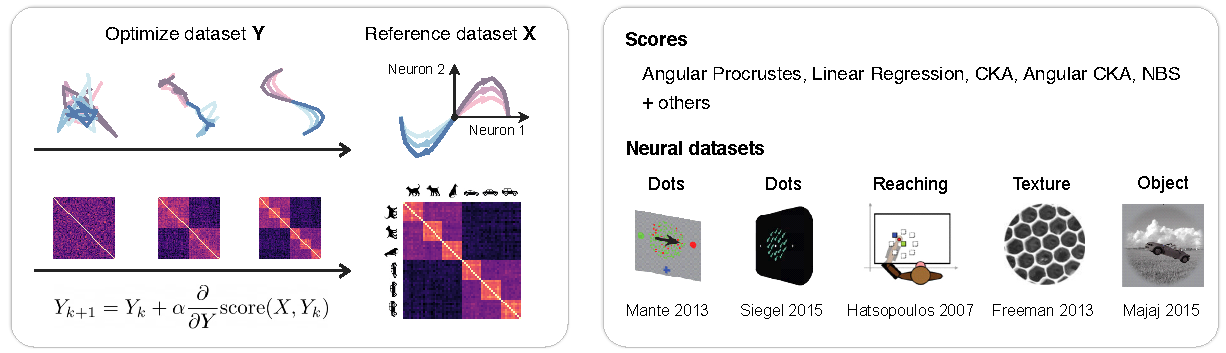
\includegraphics[width=0.99\textwidth]{figures/intro_fig.pdf}
    \caption{\textit{(a)} \textbf{To better understand the properties of similarity measures we optimize synthetic datasets to become more similar to a reference dataset}, for example, neural recordings. \textit{(b)} We analyzed similarity scores between artificial datasets and electrode recordings from five experiments on nonhuman primates spanning a diverse range of behaviors and brain regions. } 
    \label{fig:1}% To reference this figure in the main text use Figure \ref{fig:1}
    \myspaceafterfigures
\end{figure}


\section{Introduction} \myspaceaftersections

% the current intro is specific to neuroscience, maybe we want to make it also adapted to machine learning
% see "The Platonic Representation Hypothesis" for recent work that uses similarity measures in machine learning
%\citep{huh2024platonic} Representational convergence
% different network architectures, different training objects, different datasets all eventually converging to the same representations as models get bigger and better?

%Natural intelligence entails the interactions between many systems - such as different sensory, memory, and motor systems. Therefore, ultimately, many of the open questions in systems neuroscience will require models that bridge these systems. However, there are many challenges as we work towards these multi-system models of the brain. We need guidance to search through this huge design space of potential models. It would be helpful to have metrics for comparing models and brains, that allow us to extract general design principles, or alternatively, highlight the power of heterogeneity, and shine a spotlight on aspects of the biological solution space that are currently furthest from our existing models. 
%combinations of tasks and brain regions that are not currently well explained with existing models.
%It would be helpful to have metrics comparing models and brains, that allow us to extract general principles that are applicable across many models, or alternatively, highlight the power of heterogeneity, and shine a spotlight on combinations of tasks, datasets, and models that are not currently well explained.

Similarity measures have become a cornerstone in evaluating representational alignment across different models \citep{Kornblith2019}, different biological systems \citep{Kriegeskorte2008}, and across both artificial and biological systems. Researchers have employed diverse methods to compare model representations with, for example, brain activity, aiming to identify models that exhibit brain-like representations \citep{YaminsHong2014, Sussillo2015, SchrimpfKubilius2018, nayebi2018task}. However, while these measures are actively used and provide an efficient way to compare structure across complex systems, it is not clear that they adequately represent the computational properties of interest, and there is a need to better understand their limitations. Whenever we choose a similarity measure, we are making a commitment to what we care about in the two systems we are comparing. Therefore, understanding what drives these similarity scores is crucial for understanding this commitment. The field lacks clear guidelines for interpreting similarity scores in a given experimental context.%Therefore, understanding the properties of these similarity measures is crucial for understanding this commitment. The field lacks clear guidelines for selecting the most appropriate measure for a given context.

%\citep{Conwell2022} More pessimistic view about the approach. "We highlight that standard model-to-brain linear re-weighting methods may be too flexible, as most performant models have very similar brain-predictivity scores, despite significant variation in their underlying representations"

In this work we study several popular methods that have been proposed to quantify the similarity between models and neural data, in particular, linear regression \citep{YaminsHong2014, SchrimpfKubilius2018}, Centered Kernel Alignment (CKA) \citep{Kornblith2019}, angular Procrustes distance \citep{Williams2021, ding2021grounding}, and Normalized Bures Similarity (NBS) \citep{tang2020similarity}. See appendix \ref{appendix:measures} for a brief overview. We analyzed neural data from studies on nonhuman primates (Figure \ref{fig:1}) and compared the neural responses to task-optimized recurrent neural networks (RNNs), or synthetic datasets, with different similarity scores. In order to study what drives high similarity scores we directly optimize the synthetic datasets to maximize their similarity to the neural datasets as assessed by different similarity measures.% different methods, for example, linear regression, CKA, or angular Procrustes distance. 

%Comparing similarity scores across studies is challenging, primarily due to variability in naming and implementation conventions. As part of our contribution to the research community we have created, and are continuing to develop, a \textit{Python package} that benchmarks and standardizes similarity measures.% Can remove this last sentence if we introduce a Main Contributions section

%We analyzed neural data from five studies on nonhuman primates.

% talk about RNN figure here instead of in the results section?
\textbf{Disagreement between similarity measures.}
An example application of similarity measures is to quantify how brain-like models are. However, when we compare task-optimized RNNs to two neural datasets, as shown in Figure \ref{fig:rnn}, we find that different similarity measures do not agree about which models are more similar to the data, or even about whether the models are more or less similar than two baseline scores that compare modified versions of the neural data to the original neural data.  Are most of the models generally performing well or not, i.e. achieving model-data similarities above one or both of these baseline scores? Different measures give different answers. These similarity measures lack consistency and do not present a consensus interpretation. This is not an irrelevant exercise as all of these similarity measures have been used in the literature to compare models to neural data.

%An example application of similarity measures is to quantify how brain-like models are. Prior work in vision has shown similarities between task optimized neural networks and recordings from visual areas \citep{SchrimpfKubilius2018, nayebi2018task} using the linear regression similarity measure. However, when comparing multiple similarity measures, we find disagreement and lack of consistency.  Different measures tell different stories. No consensus. Figure \ref{fig:rnn}


Our main \textbf{contributions} and findings can be summarized as follows:
\begin{enumerate}
\item We show that a good value for a similarity score varies depending on the similarity measure and the dataset (Figure~\ref{fig:3}). Furthermore, we demonstrate that a high similarity score does not \textit{guarantee} that models encode task-relevant information in a manner consistent with neural data. This is particularly relevant for the many studies that rely on these similarity measures to quantitatively characterize the degree of alignment between models and brains.

\item We identify what drives high similarity scores by differentiating through the similarity measures to directly maximize the score. We discover that different similarity measures differentially prioritize learning principal components of the data. For example, CKA, as opposed to angular Procrustes, may indicate a high score when many of the lower variance components are not captured, even when these dimensions carry crucial task-related information (Figures~\ref{fig:4} and \ref{fig:5}).%For example, CKA, as opposed to angular Procrustes, may indicate a high score when much of the data variance is not captured, even when these lower variance dimensions carry crucial task-related information (Figures~\ref{fig:4} and \ref{fig:5}).

\item Through theoretical derivation we show the sensitivity of CKA, angular Procrustes, and Normalized Bures Similarity to the variance of principal component dimensions, and explain the dependence CKA shows to high variance components (section \ref{theory_nbs_cka} and Figure~\ref{fig:theory_all_datasets})

\item We characterize the allowable range of scores between two different similarity measures by jointly optimizing their scores. Surprisingly, we reveal that a high angular Procrustes similarity implies a high CKA score, but not the converse (for the dataset shown in Figure~\ref{fig:joint_optim}).

\item Comparing similarity scores across studies is challenging, primarily due to variability in naming and implementation conventions. As part of our contribution to the research community we have created, and are continuing to develop, a Python package that benchmarks and standardizes similarity measures. Currently there are approximately 100 different similarity measures from 14 packages.
\textbf{Similarity package:} 
\href{https://github.com/nacloos/similarity-repository}{https://github.com/nacloos/similarity-repository}
% \href{https://github.com/diffscore/similarity-repository}{https://github.com/diffscore/similarity-repository}



\end{enumerate}

\iffalse% begin multiline comment
\textbf{Main contributions}:
\begin{enumerate}
\item  A general method to characterize and compare similarity measures on experimental datasets
\item We show in both theory and simulations how these scores change when different principal components are perturbed
\item Comparing similarity scores across studies is challenging, primarily due to variability in naming and implementation conventions. As part of our contribution to the research community we have created, and are continuing to develop, a \textbf{Python package} that benchmarks and standardizes similarity measures\footnote{https://anonymous.4open.science/r/similarity-repository-03D3}.

    TODO: give numbers
    15 backends (papers)
    106 metrics
    1 package, 1 api
        
\end{enumerate}
\fi% end multiline comment

% Took inspiration from best paper awards for the structure of the paper (bold, italitc, bullet points, etc.)
% https://proceedings.neurips.cc/paper_files/paper/2023/file/9d89448b63ce1e2e8dc7af72c984c196-Paper-Conference.pdf
% https://proceedings.neurips.cc/paper_files/paper/2023/file/adc98a266f45005c403b8311ca7e8bd7-Paper-Conference.pdf
% https://openreview.net/pdf?id=HPuSIXJaa9

% TODO: add figure for RNN comparison to neural data for different metrics so that people can cite our work (instead of our CCN "paper")

\begin{figure}[h]
    \centering% to avoid extra vertical space use \centering instead of \begin{center} and \end{center}
    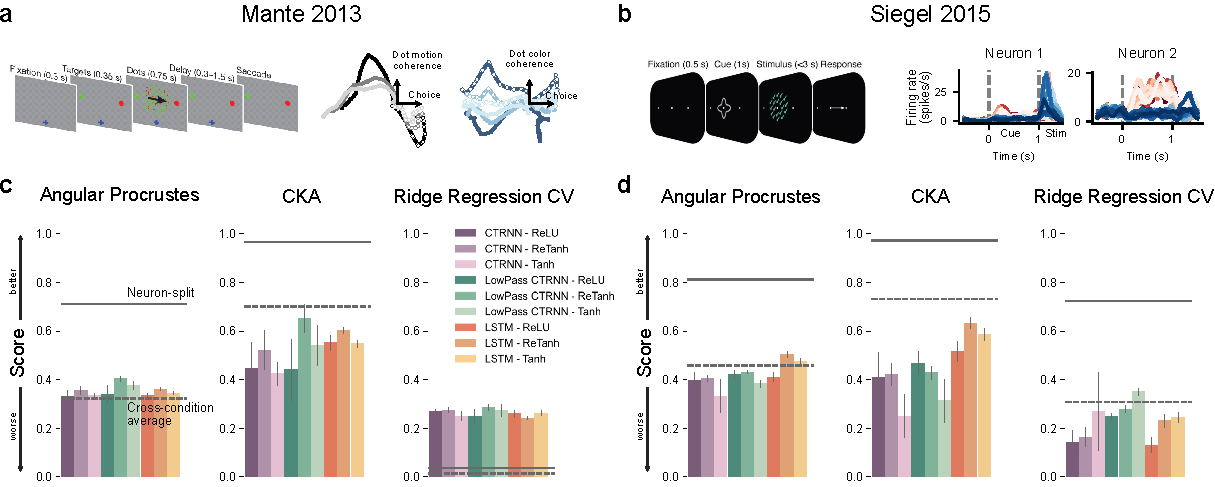
\includegraphics[width=\textwidth]{figures/rnn_bar_plots.pdf}
    \caption{%\textbf{We compare task-optimized Recurrent Neural Network models against two neural dataset with various similarity measures.} 
 \textbf{Different similarity measures do not agree on the relative rankings when comparing models to neural datasets.} One example application of similarity measures is to evaluate the similarity of task-optimized recurrent neural networks to neural datasets. 
 We consider two neural datasets from \textit{(a)} prefrontal cortex (PFC) \citep{Mante2013} and \textit{(b)} Frontal Eye Field (FEF) \citep{Siegel2015} in monkeys performing an experimental task that required the animal to attend to either color or motion information while ignoring the non-cued feature of the stimuli. \textit{(c, d)} RNNs with three different architectures, CTRNN, LowPassCTRNN, LSTM and three different nonlinearities, ReLU, ReTanh, Tanh are compared to neural datasets (see appendix \ref{appendix:models_and_datasets} for details).
 % We compare task-optimized recurrent neural networks to neural datasets. 
 % \textbf{Different similarity measures are not consistent when comparing task-optimized recurrent neural networks to neural datasets.} We consider two neural datasets from prefrontal cortex (PFC) \citep{Mante2013} \textit{(a)} and Frontal Eye Field (FEF) \citep{Siegel2015} \textit{(b)} in monkeys performing an experimental task that required the animal to attend to either color or motion information while ignoring the non-cued feature of the stimuli. 
 % On each trial, a field of colored moving dots is shown.  Monkeys are given a cue at the beginning of the trial to determine whether the dots in the stimulus are moving left vs right, or are red vs green. The monkey reported its choice with a saccade to one of two visual targets. In both datasets, we analyzed neural activity taken when the dot stimulus was presented. In panel \textit{a} neural activity is visualized in a low-dimensional space capturing task-relevant dynamics using the targeted dimensionality reduction method from Mante et al. 2013. Each curve shows the average neural activity for a different experimental condition. See Mante et al. 2013 for a detailed description of the analysis. This visualization highlights features of the data but the similarity scores were computed using the firing rates from the electrode recordings before any dimensionality reduction. In panel \textit{b} neural firing rates for two example neurons are shown with the colors denoting average activity for different experimental conditions. 
 % \textit{(c, d)} RNNs with three different architectures, CTRNN, LowPassCTRNN, LSTM and three different nonlinearities, ReLU, ReTanh, Tanh are compared to neural datasets. 
 % The Neuron-split baseline score was obtained by dividing the neurons from a single dataset into disjoint sets and then comparing. If the model-data scores are equal to the neuron-split scores this indicates that model activity is indistinguishable from the neural activity of other recorded neurons. 
 % The Condition-average baseline score was obtained by averaging the neural activity along the trial and condition dimensions and comparing it to the original dataset. Each neuron in this condition-averaged dataset still has a unique time-varying firing rate. This strong baseline shows the similarity to the original data that one can obtain by only keeping the condition-independent neural dynamics. \textbf{The different similarity measures do not agree on the relative rankings of the models, or on a more global scale, how similar the models are relative to the two baseline scores.}
 }
    \label{fig:rnn}% To reference this figure in the main text use Figure \ref{fig:rnn}
    \myspaceafterfigures
\end{figure}

\section{Related Work}  \myspaceaftersections
% could go in intro instead
\textbf{Reviews.} Recent reviews by \citet{sucholutsky2023getting} and \citet{klabunde2023similarity}  provide comprehensive overviews of representational similarity measures and their theoretical properties. While these reviews highlight the diversity of available metrics, they offer limited practical guidance on interpreting similarity scores.%While these reviews highlight the diversity of available metrics, they offer limited practical guidance on metric selection.


Our work addresses this gap by proposing a general framework for evaluating similarity measures. By directly optimizing synthetic datasets to maximize their similarity to, for example, neural recordings, we can systematically investigate how different metrics prioritize various aspects of the data, such as specific principal components or task-relevant information. %Our work addresses this gap by proposing a general framework for comparing similarity measures on experimental neural datasets. 
%By directly optimizing synthetic datasets to maximize their similarity to neural recordings, we can systematically investigate how different metrics prioritize various aspects of the data, such as specific principal components or task-relevant information.
Similarity measures are often characterized by the invariance properties between representations with maximum similarity. In contrast, we focus on what drives intermediate similarity scores and how to interpret them, since we are often dealing with intermediate levels of similarity in practice when comparing models to brain data.

\textbf{Mathematical properties.} This work builds upon several important theoretical and empirical contributions. \citet{Kornblith2019} discussed the invariance properties of similarity measures and their implications for comparing neural representations. \citet{Williams2021} advocated for similarity measures that satisfy the axioms of a metric distance. \citet{harvey2023duality} established a duality between Normalized Bures Similarity (NBS) and Procrustes distance, shedding light on their mathematical relationship to CKA. We leverage these theoretical insights to provide a deeper interpretation of our empirical findings.

%\textbf{Issues with CKA.} \citep{ding2021grounding, davari2022reliability, murphy2024correcting}

%\citep{Han2023} linear regression and CKA fail to identify architectures.


\textbf{Comparison with functional measures.} Our approach shares similarities with the work of \citet{ding2021grounding}, who evaluated metrics based on their correlation with functional behavioral measures.
They analyzed a collection of trained models and observed how variations in the models, such as the removal of principal components, impacted both the similarity scores and the performance on task-specific probes. 
They identified that CKA exhibited sensitivity primarily to the top principal components, while orthogonal Procrustes demonstrated more robust performance.

% TODO: still requires some work
However, our approach differs significantly in how we construct a diverse set of datasets with varying behavioral characteristics. 
Instead of relying on pre-trained models, we begin with unstructured noise and directly optimize it to maximize similarity to neural recordings. 
This allows us to address questions such as whether high similarity scores can be achieved without encoding task-relevant variables.
Our optimization-based approach reveals how different similarity measures guide the emergence of task-relevant information within the synthetic datasets, offering a dynamic perspective on their properties. Additionally, by leveraging our optimization-based perspective for multiple similarity measures we can find the allowable ranges of scores, and identify dependencies between similarity measures.

In contrast to the majority of previous work, our method is model-agnostic, focusing on the properties of similarity measures themselves rather than specific model architectures. 
% TODO: similar to SueYeon's paper on spectral bias in linear regression \citep{Canatar2023}, but they only analyze linear regression. Here general framework applicable to any differentiable metric.
We demonstrate the generalizability of our findings by applying our framework to multiple neural datasets, revealing consistent patterns in how different metrics prioritize data features. Interestingly, we find that the optimization dynamics observed with neural data are closely predicted when using Gaussian datasets with matched variance distributions. This suggests that our insights extend beyond the specifics of individual neural datasets and reflect fundamental properties of the similarity measures themselves.


% Similarity measures are commonly used methods to evaluate representational alignement between different systems. For example, between models and brain datasets \citep{SchrimpfKubilius2018} \citep{nayebi2018task}.  
% Many different similarity measures have been proposed.  \citet{sucholutsky2023getting} and \citet{klabunde2023similarity} have recently reviewed representational similarity measures used in the literature,  as well as their properties. Yet little guidance about how to choose which metric to use in practice.

% Here we propose a general approach to compare similarity measures on neural datasets.
% We use behavioral measures to compare with similarity scores of different measures.

% Recent work on better characterizing the mathematical properties of similarity measures such as their invariance properties \citep{Kornblith2019, Williams2021} Metrics should satisfy axioms of metric distance.
% \citep{harvey2023duality}  showed a duality between NBS and Procrustes distance, and how it relates to CKA. We further show here how this connection can be used to better understand our experimental findings.

% Our approach is closely related to the approach proposed by \citet{ding2021grounding}. They evaluate metrics based on how well they correlated with other functional/behavioral measures.
% For example they evaluate different metrics on datasets when deleting principal components (PCs) and evaluating how it correlates with task specific probing metrics.
% They found results very similar to ours. CKA sensitive only to the first PCs while orthogonal Procrustes performs best. TODO: other papers showing issues with CKA

% Our approach is not just based on correlation, where models high task decoding accuracy are also observed to have high similarity score. Here we show that, starting from unstructured noise, optimizing for similarity causes structure to be created in the noise, which progressively encode task relevant information.  
% TODO: explain how what they do is not enough

% how our method is different and novel
% Here our method doesn't require any models, model agnostic
% We apply it on several neural datasets. However, our findings are mainly the same across datasets. Maybe they tell us something about the measures, independently of the neural dataset. Especially with our result that optimization dynamics are well predicted by replacing the neural dataset by a Gaussian dataset with same spectrum.

% From the Ding2021 paper: "Unfortunately, popular metrics fail at least one of these two tests. CCA is not specific random initialization noise overwhelms differences between even far-apart layers in a network (Section 3.1). CKA on the other hand is not sensitive, failing to detect changes in all but the top 10 principal components of a representation"
% "Meanwhile, the Orthogonal Procrustes distance, a classical but often overlooked2 dissimilarity measure, balances gracefully between CKA and CCA and consistently performs well."
% From their discussion: "In contrast to the squared distance of Orthogonal Procrustes, CKA actually reduces to a quartic function based on the dot products between the squared entries of Λ1 and Λ2. As a consequence, CKA is dominated by representations’ largest singular values, leaving it insensitive to meaningful differences in smaller singular values"
% "Our procedure requires choosing a collection of models S; the crucial feature of S is that it contains models with diverse behavior according to f . Different sets S, combined with a functional difference f , can be thought of as miniature “benchmarks" that surface complementary perspectives on dissimilarity measures’ responsiveness to that functional difference"
% They take S as different sets of trained models.
% Since Orthogonal Procrustes performed well on most of our tasks, it could be a promising foundation for a new measure, and recent work shows how to regularize Orthogonal Procrustes to handle high noise (Pumir et al., 2021).



\section{Method} \myspaceaftersections

\subsection{Measuring similarity}
% \subsection{Similarity measures} % don't need it if only one subsection
To evaluate the similarity of representations between two systems, we extract feature representations such as activity in a brain area or model layer in response to some sample stimuli. Our objective is to quantify the alignment between these representations using a similarity score. Assume two datasets $X$ and $Y$ represent these features with dimensions (sample, feature) and mean-centered columns. Datasets with temporal dynamics are reshaped from (time, sample, feature) to (time*sample, feature). We define a scoring function $\text{score}(X, Y)$ as a measure that increases with similarity, achieving a maximum of 1 when $X = Y$. 

We consider the following similarity measures (see appendix \ref{appendix:measures} for details):
\begin{itemize}
    \item \textbf{Centered Kernel Alignment (CKA)} measures the correlation between the kernels of two datasets $X$ and $Y$ \citep{Kornblith2019}. We consider here linear CKA where the kernels are $XX^T$ and $YY^T$.
    % $$\text{CKA}(X, Y) = \dfrac{\| X^T Y \|^2_F}{\| X X^T \|_F \| Y Y^T \|_F}$$
    $$\text{CKA}(X, Y) = \dfrac{\langle \text{vec}(XX^T), \text{vec}(YY^T) \rangle}{\|XX^T\|_F \| YY^Y\|_F}$$

    \item \textbf{Angular CKA} is a variant of CKA that satisfies the axioms of a distance metric \citep{Williams2021, lange2022neural}. It is defined as the arccosine of CKA. We additionally renormalize it to have a value between 0 and 1, where 1 is perfect similarity.
    % The CKA score varies between 0 and 1, where 1 corresponds to perfect similarity. We consider as well another variant of CKA which is the arccosine of CKA. As \citep{Williams2021} showed, this gives a measure of distance, where 0 corresponds to perfect similarity, that satisfies the axioms of a metric, e.g. the triangle inequality. This metric has been also called Angular CKA as \citep{lange2022neural}. Here we normalize this meause to have a measure of similarity between 0 and 1 so that it can directly be compared to other scoring methods. We do that by first normalizing the angular distnace between 0 and 1 by dividing by pi over 2, and then substract the result from 1 to have a measure that increases with similarity.
    % $$\text{AngularCKAScore}(X, Y) := 1 - \dfrac{\arccos (\text{CKA}(X, Y))}{\pi / 2}$$
    
    \item \textbf{Angular Procrustes} finds the optimal orthogonal linear alignment between $X$ and $Y$ to maximize their correlation \citep{Williams2021, ding2021grounding}.
    $$\min_{Q \in \mathcal{O}} \text{arccos} \dfrac{\langle X, QY\rangle}{\|X\|_F \|Y\|_F}$$
    where $\mathcal{O}$ is the group of orthogonal linear transformations. \citet{Williams2021} proposed taking the arccosine to satisfy the axioms of a distance metric. Here we rescale the angular Procrustes distance to obtain a scoring measure between 0 and 1, where 1 is perfect similarity.

    \item \textbf{Normalized Bures Similarity (NBS)} \citep{tang2020similarity} is the cosine of the angular Procrustes distance \citep{harvey2023duality}. NBS is also closely related to CKA and mainly differs by a choice of matrix norm (see details in appendix \ref{appendix:measures}).
    $$\text{NBS}(X, Y) = \dfrac{\|X^T Y\|_*}{\sqrt{\|X X^T\|_* \|Y Y^T\|_*}}$$


    \item \textbf{Ridge Regression} finds the best linear mapping $B$ that predicts a reference dataset $X$ from a dataset $Y$ \citep{YaminsHong2014, SchrimpfKubilius2018}. We measure the goodness of fit using $R^2$ and use ridge regularization as well as 5-fold cross-validation that tests generalization across different experimental conditions. We use $\lambda = 100$ by default and show results with varying $\lambda$ in appendix \ref{appendix:additional_results}.% In this work we analyze average neural activity and so cross-validation is performed across different experimental conditions.
    $$B^* = \argmin_B \| X - YB\|^2_F + \lambda \| B \|_F$$

    $$R^2_{LR} = 1 - \dfrac{\| X - YB^*\|^2_F}{\| X \|^2_F}$$

    \item \textbf{Linear Regression.} Same as Ridge Regression but for $\lambda = 0$ (unregularized).

\end{itemize}

% Our analysis is generally applicable to any measure of similarity that is differentiable. We maintain a python package and we will keep adding more measures to the benchmark by updating the project page.
% TODO: mention similarity-repository package and how we use it to validate our implementations of the measures?


\subsection{Optimizing similarity scores}
\label{appendix:optimizing}

To better characterize similarity measures we optimize synthetic datasets $Y$ to become more similar to a reference dataset $X$. We initialize the synthetic dataset $Y$ by randomly sampling from a standard Gaussian distribution with the same shape as $X$. We use Adam \citep{kingma2017adam} to optimize $Y$ to maximize the similarity score with $X$, leveraging the differentiability of the similarity measures, and stop the optimization when the score reaches a fixed threshold near 1. % We stop the optimization when the scores reaches a threshold of 0.995.
% added based on the rebuttals:
Note that some similarity measures have parameters to optimize to compute the similarity score. Our method can be applied in such cases too, as long as the similarly score is differentiable with respect to the input datasets. For example, in the case of linear regression, we directly differentiate PyTorch's lstsq function.
% In this case, there are two things being optimized. First, we use PyTorch’s lstsq function to compute the linear regression score. Then, we use PyTorch’s Adam optimizer to optimize the synthetic data, leveraging the differentiability of the lstsq function. 
% From the reviewer: "Presumably there are two things that get optimized: the linear regression parameters themselves, and the synthetic data used as regressors."

As we optimize $Y$ towards greater similarity with $X$, we simultaneously evaluate how well task-relevant variables can be linearly decoded from the evolving synthetic data. This decoding analysis employs logistic regression with stratified 5-fold cross-validation. For datasets with temporal dynamics, we fit a separate decoder for each time step and report the average accuracy across time.
% To analyze the optimized synthetic datasets, we evaluate how well task variables can be linearly decoded with cross-validated logistic regression. We fit a different decoder for each time step and cross-validate using Stratified K-Folds with 5 folds. The reported decoding accuracy is the test accuracy averaged across all time steps and across the 5 folds.

We also evaluate how each principal component (PC) of the reference dataset $X$ is captured as $Y$ is optimized for similarity. Specifically, for each PC $v_i$ of $X$, we use linear regression to find the optimal linear combination of columns of $Y$ that best predicts $Xv_i$. The goodness of fit is then quantified using the $R^2$ coefficient:
$$R_{PC_i}^2:= 1 - \dfrac{\| (X - \hat{X})v_i \|^2}{\|Xv_i\|^2}$$
where $\hat{X} = Y\hat{B}$ and $\hat{B} = \text{argmin}_B \| X - YB\|^2_F$.

% All experiments were conducted on a NVIDIA GeForce GTX TITAN X and required less than a day of compute time.



\section{Results} \myspaceaftersections
% in intro or here?
% \subsection{Disagreement of similarity scores across metrics}
% Different measures seem to be telling different stories. No concensus.



% \subsection{High similarity scores do not guarantee encoding of task relevant variables}
\subsection{What constitutes a good similarity score depends on the similarity measure and the dataset}

\textbf{What is a good value for a similarity score?}
Our approach to address this question is to examine, across five neural datasets, the similarity score required for a synthetic dataset to encode task relevant information to the same degree as the neural data.
% We start by asking if synthetic datasets with high similarity scores relative to the neural data, encode task relevant variables, for example, the stimulus features or the response of the monkey, in the same way as the neural data. More specifically, is it possible for the synthetic datasets to have a high similarity score while failing to encode task relevant variables? 
% There are many ways this can be approached but what we’ve done here, across five neural datasets, is to look at the similarity score required for a synthetic dataset to encode task relevant information to the same degree as neural data. 
More specifically, the dots along the x-axis in Figure \ref{fig:3} indicate the score when a decoder trained on the synthetic data can extract 90\% of the full task relevant information present in the neural data. Consider the Mante 2013 dataset, and notice that the “good” scores for the six similarity measures are quite different, ranging from less than 0.5 to almost 1. So even for the same dataset, the similarity score required to encode task relevant information to a similar extent as the neural data, can be very different across similarity measures.

Now if we look across the five neural datasets, at a single similarity measure, we can see that what constitutes a good score varies depending not only on the similarity measure but also on the dataset. An angular Procrustes score above 0.5 may constitute a good score for the Mante 2013 dataset but a score above 0.8 is required for the Siegel 2015 dataset (see also Supplementary Figure \ref{fig:var_decoding_supp}).

\textbf{High similarity scores do not guarantee encoding of task relevant variables.}
% We start by asking if synthetic datasets with high similarity scores relative to the neural data, encode task relevant variables, for example, the stimulus features or the response of the monkey, in the same way as the neural data. More specifically, is it possible for the synthetic datasets to have a high similarity score while failing to encode task relevant variables? 
A crucial point to make with Figure \ref{fig:3} is that high similarity scores near the maximum value of 1, particularly for CKA and unregularized linear regression without cross-validation, do not guarantee that models encode task-relevant information in a manner consistent with neural data, i.e. the CKA and linear regression curves in the Siegel 2015 dataset do not approach the horizontal line showing the decode accuracy for the neural data. There may be important features in a dataset that are not captured by a model even when the model-data similarity score is high.

For linear regression, even cross-validated and regularized, a high similarity score does not necessarily mean that the task relevant information is encoded in a similar manner to the neural data (Supplementary Figure \ref{fig:linreg_comparison}).



% \textbf{Problem with CKA and linear regression}.
% Surprisingly we find that for linear regression and CKA the answer is yes, a high similarity score does not necessarily mean the synthetic datasets encode task relevant variables like the neural data. Figures \ref{fig:2}a and \ref{fig:2}b  show the decode accuracy of a linear classifier trained to decode task relevant variables (cross-validated across different conditions) as the similarity score increases. 
% % TODO: not a binary classifer for the other datasets than Mante and Siegel
% % Before optimization, the synthetic datasets initially consisted of Gaussian noise and the decode accuracy was near the baseline chance level of 0.5 as expected for the binary classifier used in this analysis. 


% moved this paragraph to appendix
% In Figure S2 we focus on a popular similarity measure, linear regression, and show how much task relevant information can be decoded from a synthetic dataset that is optimized to become increasingly more similar to the Siegel 2015 dataset. The point here is that even when linear regression is cross-validated and regularized, a high similarity score does not necessarily mean that task relevant information is encoded in a similar manner to neural data (leftmost panels).

% We also find that linear regression, when regularized and cross-validated across experimental conditions, performs well. But it requires more care to work with and has more hyperparameters to tune than angular Procrustes, for example.


% Consider the synthetic data optimized towards the Siegel 2015 neural recordings using CKA similarity (second row and column in Figure \ref{fig:2}). When the synthetic dataset has a high similarity score of 0.9 the decode accuracy for all the task variables is still less than that found in the neural activity (horizontal dashed lines). This is in contrast to the case where synthetic data is optimized to maximize angular Procrustes similarity (first column) and a similarity score of near 0.9 yields a dataset that encodes task variables to the same degree as the neural recordings. Note that both CKA and angular Procrustes have the same similarity scale ranging between 0 and 1 (perfect similarity). See appendix \ref{appendix:measures} for more details. 

% As another example, consider the decode accuracy for the color of the stimulus that was shown in the experiments (green curves). For linear regression and CKA the similarity score can be high even when the data does not encode this task variable at the level found in the neural activity, suggesting there is a mismatch between the datasets with a high similarity score and features of the neural activity. In contrast, for the angular Procrustes distance the synthetic datasets that have a high similarity score relative to the neural activity also encode the task relevant variables.%Consider the decode accuracy for the color of the stimulus that was shown in the experiments (green curves). For linear regression and CKA the similarity score can be high while the decode accuracy is still less than that found in the neural data (horizontal dashed lines), suggesting there is a mismatch between the datasets with a high similarity score and features of the neural data. In contrast, for the Procrustes distance the synthetic datasets that have a high similarity score relative to the neural data also encode the task relevant variables.

% this is now the main message of this section instead of being an additional note
% \textbf{How high should a good score be?} As a final more optimistic note, for all the similarity measures, we can see a general trend that optimizing the synthetic data towards higher similarity eventually leads the data to encode task relevant variables above the baseline chance level of 0.5 accuracy. One perspective on this decoding analysis is that it gives a window into what is a \textit{high} similarity score. If a high score is one where the data is encoding task relevant variables then these similarity numbers will need to be \textit{interpreted differently} based on the similarity measure.


% \textbf{High variability in the condition average baseline across metrics}. A specific number for the similarity score, 0.9 for example, can have different interpretations depending on the measure that is used, as we have seen in the examples above contrasting CKA and angular Procrustes. Conversely if two models or datasets are compared then this comparison may result in different scores depending on the similarity measure. Prior work has used the \textit{condition average baseline} as a reference score for benchmarking models against neural data \citep{Cloos2022}. The condition average baseline is obtained by averaging each neuron’s activity across trials from all experimental conditions, while still allowing each neuron to have its own unique time-varying firing rate, and then comparing this condition-averaged dataset to the original neural data. This baseline shows the similarity one can obtain by discarding the condition specific activity to keep only the condition independent dynamics of the neural activity. The condition average baseline is shown in Figures \ref{fig:2}a and \ref{fig:2}b as vertical dashed lines. For a single dataset, we are always comparing the same two quantities to obtain the condition average baseline but the scores are quite different depending on the similarity measure.
% For the angular Procrustes measure, as opposed to the linear regression similarity measure, this baseline score is closer to the point where task relevant information starts to be encoded.


%TODO: add a comment on the decode accuracy sometimes higher in optimized datasets than reference datasets.
Surprisingly, in Figure~\ref{fig:3} some optimized datasets encode task relevant information better than the original neural data (colored lines showing decode accuracy are above the horizontal dashed line). This might suggest that the optimized datasets are denoised versions of the original data. We tested this hypothesis by removing low-variance principal components from the neural dataset, but this did not change the results. This suggests it is probably a more complex form of denoising and would require further investigation (Supplementary Figure \ref{fig:task_var_decoding_pca}).


\begin{figure}[h]
  \centering% to avoid extra vertical space use \centering instead of \begin{center} and \end{center}
    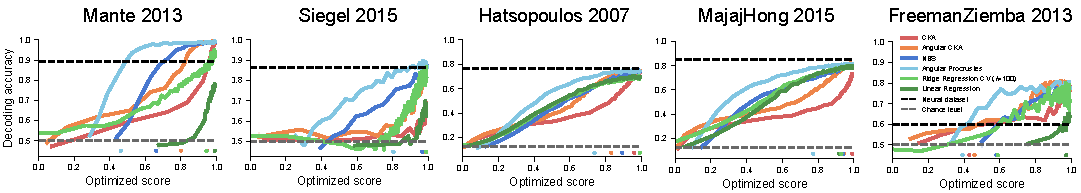
\includegraphics[width=\textwidth]{figures/task_var_decoding.pdf}
    \caption{
    \textbf{What constitutes a good score varies depending on the similarity measure and the dataset.} 
    Decode accuracy for experimental variables versus similarity scores. The experimental variables are color vs motion contexts (binary variable) for Mante 2013 and Siegel 2015, reaching direction (total of 8 directions) for Hatsopoulos 2007, object categories (total of 8 categories) for MajajHong 2015, and texture vs noise categories (binary variable) for FreemanZiemba 2013. Horizontal dashed lines show the decode accuracy from the neural data (upper line) and chance level (lower line). %See details in the respective references. 
    Colored dots above the x-axis indicate the similarity scores when the decode accuracy reaches 90\% midway between chance level and the decode accuracy from the reference neural dataset.} 
    \label{fig:3}% To reference this figure in the main text use Figure \ref{fig:3}
    %\vspace{-0.4cm}
\end{figure}


\subsection{Optimization dynamics of similarity scores}
\subsubsection{Low-dimensional synthetic datasets}
\textbf{Question.} How much of the neural data must be captured by a synthetic dataset or model before the decode accuracy reaches the level seen in the neural dataset itself? One perspective on this question is to decode the task variables from neural data after projecting onto principal components 1 through N, where principal component 1 captures the most variance. As we might expect, in order to capture all the information about the task variables, at least several principal components must be included in the decode (Figures \ref{fig:var_decoding_supp}c and \ref{fig:var_decoding_supp}d show an example of this analysis for two of the neural datasets). This motivates the following hypothesis. 



\textbf{Hypothesis.} Perhaps the reason that some variations of linear regression and CKA similarity scores can be so high while the synthetic data fails to encode task variables is because these similarity measures preferentially rely on the top few principal components. In other words, if these measures only encode information from the top principal components then this may not be sufficient to encode all the task variables. We explore this hypothesis in the following set of analyses with a synthetic dataset based on the neural recordings from Mante et al. 2013. 


\begin{figure}[h!]
\begin{center}
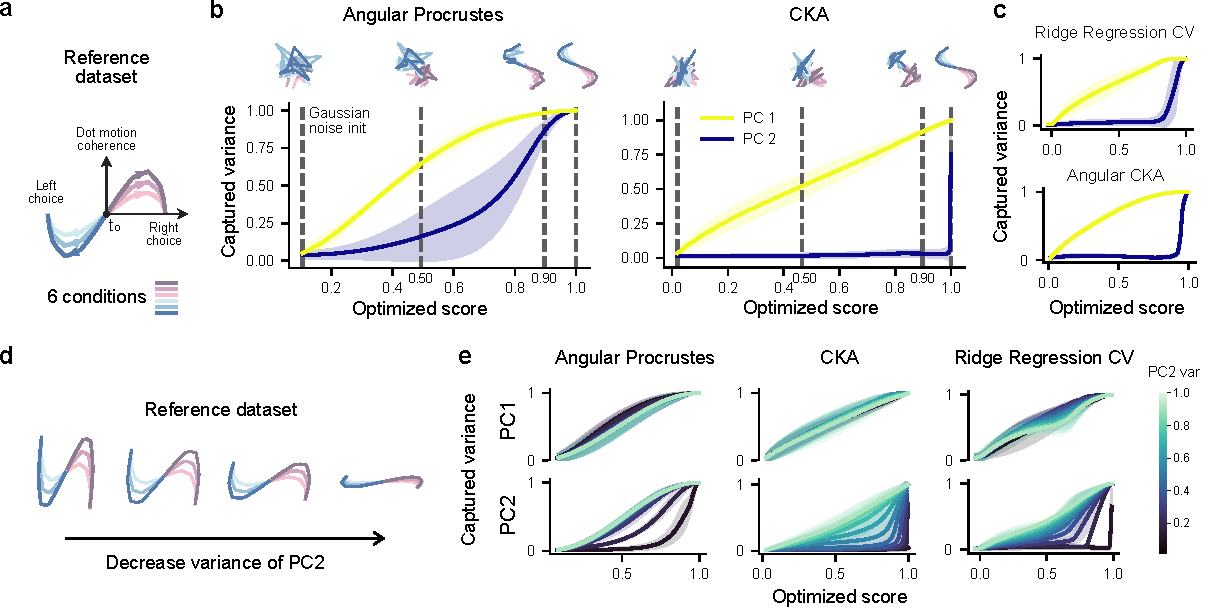
\includegraphics[width=\textwidth]{figures/opt_dynamics_toy_dataset.pdf}
%\framebox[4.0in]{$\;$}
\end{center}
\vspace{-0.2cm}% CAN DELETE! INSERTED TO MEET 10 PAGE REQUIREMENT
\caption{\textbf{Different similarity measures differentially prioritize learning principal components of the data.} \textit{(a)} Reference dataset used as a target during optimization. \textit{(b, c)} Initial Gaussian random noise data is updated to maximize similarity with the reference dataset, as quantified by one of the similarity measures. The transformation of the random noise dataset is shown at the top of panel \textit{b}. The first principal component of the reference dataset is increasingly well captured by the optimized data as the similarity scores increase (yellow curves). \textbf{The second, lower variance, component is also learned when maximizing the angular Procrustes similarity but is only captured at high similarity scores when maximizing linear regression, CKA, and angular CKA similarity.} \textit{(d)} Four reference datasets with decreasing variance along the second principal component. \textit{(e)} Similarity measures capture both principal components when their variance is approximately equal. However, when the variance differs, CKA and linear regression preferentially neglect the low variance component (curves colored according to asymmetry of variance distribution).}%However, when the variance differs, CKA and linear regression have a much more pronounced preference for learning the high variance component as opposed to angular Procrustes which causes the optimized dataset to also capture the low variance dimension (curves colored according to asymmetry of variance distribution).}
\label{fig:4}% To reference this figure in the main text use Figure \ref{fig:4}
\myspaceafterfigures
\end{figure}

\textbf{Figure \ref{fig:4}a} shows the reference dataset (compare to Figure \ref{fig:rnn}a). We can think of this reference dataset as a low-dimensional neural trajectory summarizing the population activity of many neurons, or alternatively, as the firing rates of two neurons over time (shown here encoding the two task variables of choice and dot motion coherence), recorded during six different experimental conditions, with the color in Figure \ref{fig:4}a denoting the condition. \textbf{Figure \ref{fig:4}b} shows the transformation of an initially random Gaussian noise dataset as it is optimized to maximize either the angular Procrustes or CKA similarity score with respect to the reference dataset. The score increases from an initial value near 0 to a maximum near 1 as optimization progresses, with the insets at the top of the figure showing the optimized noise dataset at various points during this procedure. The yellow curve shows how well the optimized dataset captures the first principal component of the reference dataset, as quantified by $R^{2}$, throughout optimization (see section \ref{appendix:optimizing} for details). %Notice that the second principal component, shown in purple, is captured much later during training for CKA versus Procrustes, and only at a much higher optimization score. 
Notice that the second principal component, shown in purple, is only captured at a \textit{much higher} optimization score for CKA versus angular Procrustes. \textbf{Figure \ref{fig:4}c} shows the same results when a synthetic Gaussian noise dataset is optimized towards the reference dataset using either linear regression similarity or angular CKA similarity \citep{Williams2021}.



\textbf{Dependence on the variance distribution.} The optimization dynamics not only depend on the similarity measure but also on the variance distribution of the reference dataset. Figure \ref{fig:4}d shows four reference datasets with the same variance along the first principal component but decreasing variance along the second. If both dimensions have approximately equal variance then angular Procrustes, CKA, and linear regression will learn both dimensions similarly during optimization as shown by the white curve in Figure \ref{fig:4}e. The curves are colored to indicate the fraction of variance the second principal component has relative to the first, so 1 indicates both principal components have the same variance. As the asymmetry between the principal components grows, the optimization to maximize angular Procrustes similarity still effectively learns %prioritizes 
the lower variance principal component (first column, second row), while CKA and linear regression do not capture the second principal component of the reference dataset until much later during optimization.



\begin{figure}[h!]
    \centering% to avoid extra vertical space use \centering instead of \begin{center} and \end{center}
    % 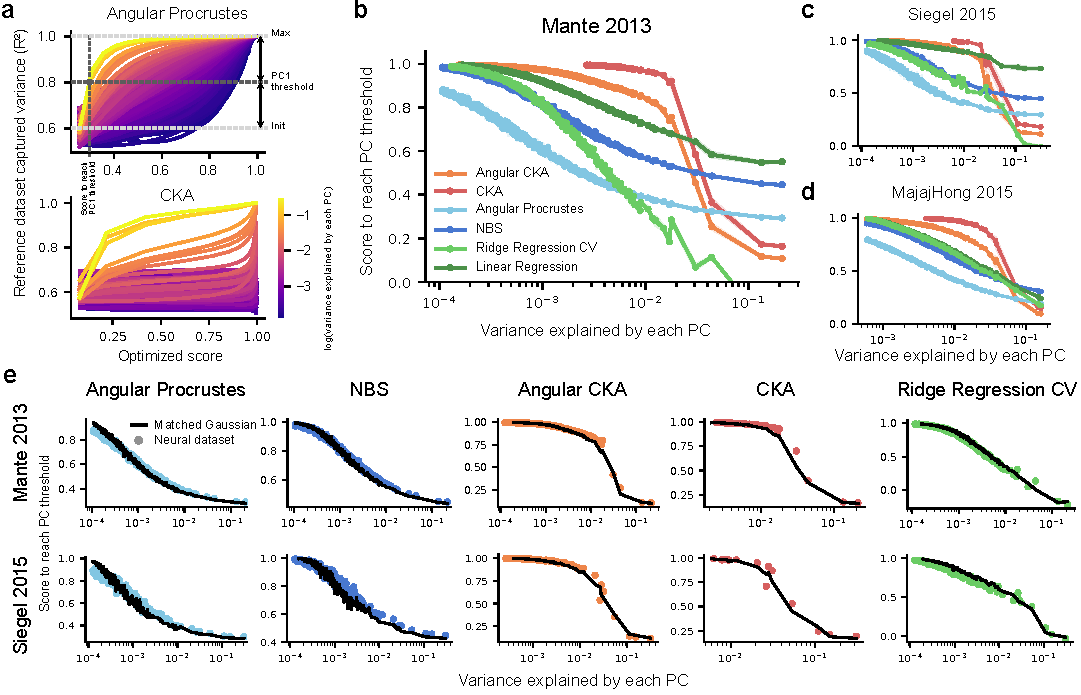
\includegraphics[width=\textwidth]{figures/captured_pc_data.pdf}
    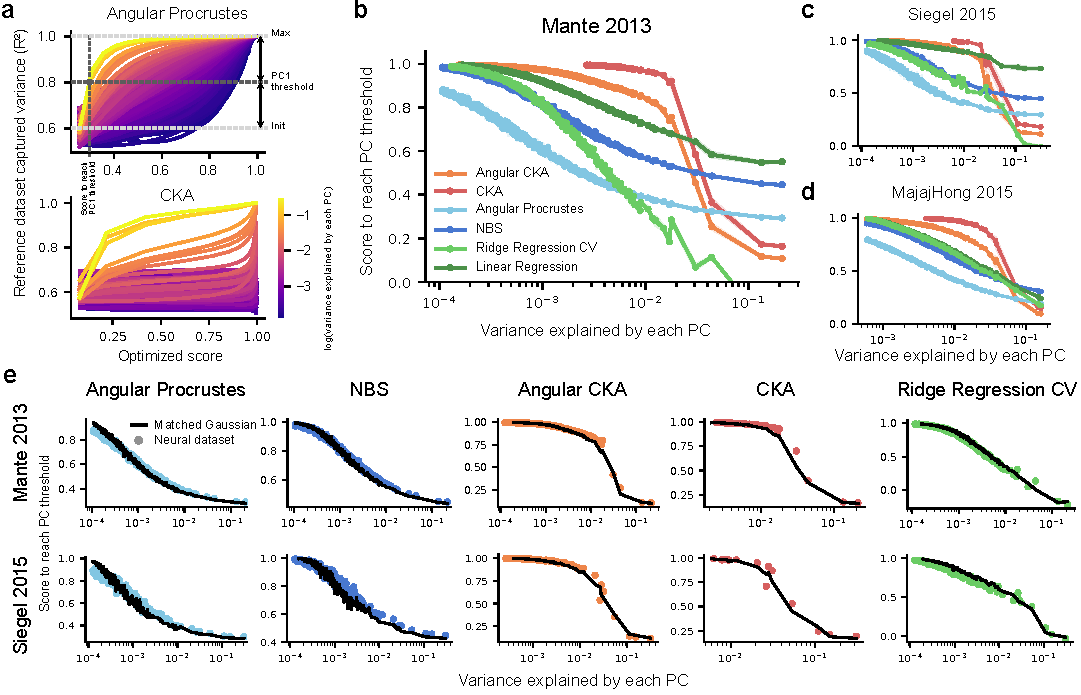
\includegraphics[width=\textwidth]{figures/captured_pc_data.pdf}
    \caption{\textit{(a)} \textbf{A randomly initialized synthetic dataset is updated to maximize the similarity with a neural dataset}, taken here to be the FEF dataset from \citep{Siegel2015}. The principal components (PCs) of this reference dataset are captured by the optimized dataset at different similarity scores, which in subsequent figures we call the score to reach the PC threshold. \textit{(b)} The score to reach the PC threshold for the \citep{Mante2013} dataset is shown as a function of the variance explained by each PC. The highest variance PC is learned first during optimization at the lowest similarity score (bottom right of figure). A vertical slice through the figure shows the similarity score required to capture a specific PC. For example, to capture the PC at $10^{-2}$ requires a much lower similarity score when maximizing angular Procrustes versus CKA (light blue curve is below the red curve). \textit{(c, d)} The reference dataset used as a target during optimization is the neural activity from \citep{Siegel2015} FEF (panel \textit{c)} and \citep{MajajHong2015} (panel \textit{d}). \textit{(e)} The neural data points are the same as in panels \textit{c} and \textit{d} (colored dots). The similarity scores at which PCs of this neural activity are learned, is well predicted by replacing neural activity with random Gaussian datasets that have a matching distribution of variances for each PC (black curves).
    % (b, c, d) Results average across 3 random seeds (important for neurips checklist)
    %\textcolor{red}{TODO: Linear regression in the plots (light green) is CV ridge regression. I'm adding the results for vanilla linear regression (dark green). Currently only shown for siegel datatset (other datasets are still running, mante should be similar to siegel but for majajhong, ridge and linear regression seems to be the same - preliminary result). We should update all the other figures and change "linear regression" by "ridge regression CV".} 
    }
    \label{fig:5}% To reference this figure in the main text use Figure \ref{fig:5}
    \myspaceafterfigures
\end{figure}


\subsubsection{Neural datasets}

The optimization dynamics revealed in Figure \ref{fig:4}a for a two-dimensional dataset also holds on real neural data (\ref{appendix:datasets}). We now consider several neural datasets as the reference dataset for the optimization procedure. Figure \ref{fig:5}a shows the optimization dynamics when a random noise Gaussian dataset is optimized towards the Siegel et al. 2015 dataset by maximizing angular Procrustes similarity (top) or CKA similarity (bottom). Each curve shows how the optimized dataset captures a single principal component of the reference dataset during the course of optimization; the yellow curve shows the highest variance component. Similar to the results in Figure \ref{fig:4}, optimizing for angular Procrustes similarity, as opposed to CKA, captures more of the lower variance components in the data for a given similarity score. 

A convenient way of summarizing these curves is to note the similarity score required to capture a given principal component above some threshold. The PC threshold is defined here (and shown in Figure \ref{fig:5}a for PC 1) as the centerpoint between the maximum and initial $R^{2}$ value for a given principal component. Figure \ref{fig:5}b shows the score required to reach the principal component threshold for the different principal components in the Mante et al. 2013 dataset. Figures \ref{fig:5}c and \ref{fig:5}d show the same curves when the reference datasets are now the electrode recordings from Siegel et al. 2015 and Majaj et al. 2015. Figures \ref{fig:5}b, \ref{fig:5}c, and \ref{fig:5}d additionally show that the metric version of CKA (angular CKA) increases CKA's sensitivity to lower variance components. 

%\textbf{Angular CKA.} \citet{Williams2021} proposed to take the arccosine of CKA to obtain a measure that satisfies the axioms of a distance metric. Figures \ref{fig:5}b, \ref{fig:5}c, and \ref{fig:5}d additionally show that the metric version of CKA (referred to as angular CKA) increases its sensitivity to lower variance components. 

\textbf{Neural curves predicted by matched Gaussians.} Surprisingly, the optimization dynamics shown in these figures are well matched when the reference neural dataset is replaced by a new reference dataset that consists of random Gaussian numbers with variances for each principal component matched to the neural data (Figure \ref{fig:5}e). The variance distribution of the reference dataset strongly determines when each principal component is captured during optimization.% \textcolor{red}{A better sentence or two about why this is interesting/important.}



\subsection{Theoretical analysis of CKA and angular Procrustes} \label{theory_nbs_cka}
% add a paragraph to motivate this section
We aim to understand the increased sensitivity of CKA scores to high variance principal components compared to angular Procrustes. Following \citet{harvey2023duality}, we use the Normalized Bures Similarity (NBS) metric as an intermediary metric between CKA and angular Procrustes. Specifically, we study the sensitivity to dimensions of different variances by analyzing the similarity scores between a neural dataset and a modified version of the same dataset when a single principal component (PC) is perturbed (Figure \ref{fig:theory_all_datasets}). We ``perturb'' a single PC of the neural dataset by first decomposing the dataset into its projections onto every PC and then replacing a single one of these projections by Gaussian random noise that is rescaled so the variance is unchanged.




\textbf{From NBS to CKA.} NBS and CKA mainly differ by a choice of matrix norm as shown in the following formulation \citep{harvey2023duality} (see appendix \ref{appendix:measures} for details):
\begin{align*}
\text{CKA}(X, Y) = \dfrac{\| X^T Y \|^2_F}{\| X X^T \|_F \| Y Y^T \|_F} && \text{NBS}(X, Y) = \dfrac{\|X^T Y\|_*}{\sqrt{\|X X^T\|_* \|Y Y^T\|_*}}
\end{align*}


% To understand the increased sensitivity to low variance principal components of NBS compared to CKA (dark blue and red curves in Figures \ref{fig:5}b, \ref{fig:5}c, and \ref{fig:5}d), we analyze their matrix norm formulation. As shown in \citet{harvey2023duality}, CKA and NBS can be formulated as follow (see appendix \ref{appendix:measures} for details):
% \begin{align*}
% \text{CKA}(X, Y) = \dfrac{\| X^T Y \|^2_F}{\| X X^T \|_F \| Y Y^T \|_F} && \text{NBS}(X, Y) = \dfrac{\|X^T Y\|_*}{\sqrt{\|X X^T\|_* \|Y Y^T\|_*}}
% \end{align*}

NBS quantifies similarity using the nuclear norm, which involves a sum of singular values, whereas CKA uses the Frobenious norm, which sums the square of the singular values. The additional square operation in CKA significantly increases the contribution of large variance components. We show this in theory by considering how CKA and NBS change when perturbing a single principal component of the data. The result is that CKA depends quadratically on the variance of the perturbed principal component, whereas NBS has a linear dependence (see proof in appendix \ref{appendix:cka_nbs_theory}).
% , as empirically validated in Figure \ref{fig:theory}a.
\begin{align*}
\text{CKA}(X, \tilde{X}_k) \approx \dfrac{\sum_{i \ne k} (\lambda_X^i)^2}{\sum_i (\lambda_X^i)^2} && \text{NBS}(X, \tilde{X}_k) \approx \dfrac{\sum_{i \ne k} \lambda_X^i}{\sum_i \lambda_X^i}
\end{align*}
where $\tilde{X}_k$ is equal to $X$ where only the $k^{\text{th}}$ principal component is modified, and $\lambda_X^i$ are the eigenvalues of $XX^T$.

We validate these results empirically by computing CKA and NBS scores between five different neural datasets and versions of these datasets when a single principal component is perturbed (see colored dots in Figure \ref{fig:theory_all_datasets}). As predicted by the theory, the NBS and CKA scores are well matched by, respectively, a linear and a quadratic function of the variance of the perturbed PC (see orange and blue curves). 


\textbf{From angular Procrustes to NBS.} \citet{harvey2023duality} showed that angular Procrustes is related to  Normalized Bures Similarity (NBS) \citep{tang2020similarity} by the arccosine function. We additionally normalize the angular Procrustes distance to obtain a score version, where 1 corresponds to perfect similarity.
$$\text{AngularProcrustesScore}(X, Y) = 1 - \text{arccos}(\text{NBS}(X, Y)) * 2 / \pi$$

The arccosine function decreases linearly around $0$ with a slope of $-1$ and has a vertical asymptote in $1$. When NBS is small, which corresponds to high variances of the perturbed PC in Figure \ref{fig:theory_all_datasets}, angular Procrustes is also linear. When NBS is around 1, which corresponds to low variances of the perturbed PC in Figure \ref{fig:theory_all_datasets}, angular Procrustes has increased sensitivity compared to NBS, as explained by the large slope of arccosine around $1$.

% The linear and the arccosine relationships explain the empirically observed differences between angular Procrustes and CKA.

% Similar to angular CKA, we find that the arccosine increases sensitivity to lower variance components (Figures \ref{fig:5}b, \ref{fig:5}c, and \ref{fig:5}d).  This can be understood by the nonlinear mapping of arccosine that expands values close to one.


% To understand the difference between Centered Kernel Alignment (CKA) and Angular Procrustes and their sensitivity to dimensions of different variance, we study, in simulation and in theory, similarity scores between a neural dataset and a modified version of the same dataset when a single principal component (PC) is perturbed. 



% We show, in simulation and in theory, that CKA is quadratic in the variance of the perturbed PC (Figure \ref{fig:theory}, blue curve), whereas NBS is linear (Figure \ref{fig:theory}, orange curve). This illustrates that CKA scores are mainly dominated by large variance PCs. Similar to NBS, Angular Procrustes is linear for large variance components (the arccosine is approximately the identity function close to 0), but is more sensitive to low-variance components than NBS (arccosine tends to infinite slope at 1) and CKA.

% TODO: do we include this?
% Note that \citet{ding2021grounding} briefly mentioned in their discussions that in the simplified case where two datasets have the same eigenvectors, CKA reduces to products of squared singular values of each dataset, whereas Procrustes distance doesn't square the singular values. This is essentially the same intuition as the result we have shown here.
% % Here we provide a more formal way to derive this result, leveraging a duality relationship discovered by \citet{harvey2023duality}. 
% % Ding2021 discussion: "In contrast to the squared distance of Orthogonal Procrustes, CKA actually reduces to a quartic function based on the dot products between the squared entries of Λ1 and Λ2. As a consequence, CKA is dominated by representations’ largest singular values, leaving it insensitive to meaningful differences in smaller singular values"



% From the rebuttals:
% This is indeed a confusing point as Figure 6a in the original paper shows results for a synthetic dataset that doesn’t have large variance PCs. We clarify this point by showing results for the 5 neural datasets in Figure S4. Specifically, CKA scores drop lower than the angular Procrustes scores when high variance PCs are perturbed (due to the quadratic dependence of CKA on the variance of the PC). Angular Procrustes is both less sensitive to high variance PCs and is more sensitive to low variance (see caption in Figure S4 for more details).


\begin{figure}[h!]
  \centering% to avoid extra vertical space use \centering instead of \begin{center} and \end{center}
    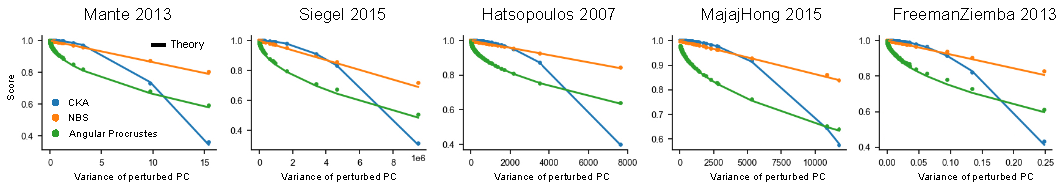
\includegraphics[width=\textwidth]{figures/theory_all_datasets.pdf}
    \vspace{-0.6cm}% CAN DELETE! INSERTED TO MEET 10 PAGE REQUIREMENT
    \caption{\textbf{The similarity score between five neural datasets and a modified version of these datasets when a single principal component is perturbed.} The colored dots show the empirical CKA, NBS, and angular Procrustes scores. The solid lines show the predictions of our theory. In particular, the CKA scores decrease quadratically with the variance of the perturbed principal component, whereas NBS scores decrease linearly. Angular Procrustes is related to NBS by the arccosine function, which explains its linear dependence to high variance PCs and its increased sensitivity to low variance PCs compared to NBS.
    % For all similarity measures, when small variance components are perturbed the similarity score is near 1. However, when high variance components are perturbed the angular Procrustes score drops much more than for CKA and Normalized Bures Similarity (NBS). 
    % To understand the difference between Centered Kernel Alignment (CKA) and Angular Procrustes and their sensitivity to dimensions of different variance, we study, in simulation and in theory, similarity scores between a neural dataset and a modified version of the same dataset when a single principal component (PC) is perturbed. We use the Normalized Bures Similarity (NBS) metric as an intermediary metric since $\text{Angular Procrustes} = 1 - \text{arccos}(\text{NBS}) * 2 / \pi$, and NBS and CKA differ only by a choice of matrix norm. We show that CKA is quadratic in the variance of the perturbed PC (blue curve), whereas NBS is linear (orange curve). This illustrates that CKA scores are mainly dominated by large variance PCs. Similar to NBS, Angular Procrustes is linear for large variance components (the arccosine is approximately the identity function close to 0), but is more sensitive to low-variance components than NBS (arccosine tends to infinite slope at 1) and CKA.
    } 
    \label{fig:theory_all_datasets}% To reference this figure in the main text use Figure \ref{fig:theory_all_datasets}
\end{figure}

\begin{figure}[h!]
    \centering% to avoid extra vertical space use \centering instead of \begin{center} and \end{center}
    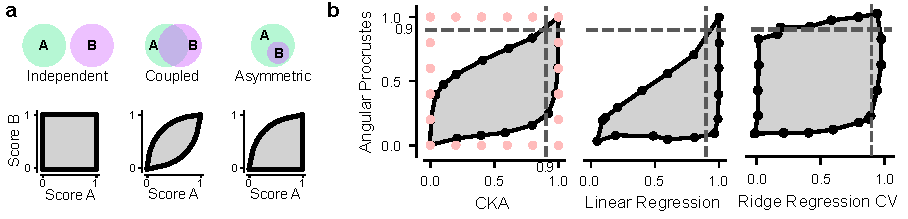
\includegraphics[width=0.9\textwidth]{figures/joint_optim.pdf}
    % (c, d): siegel15-FEF-stim_period-var99
    \vspace{-0.2cm}
    \caption{\textbf{We jointly optimized the values of both angular Procrustes and CKA or linear regression to illustrate the allowed ranges of both similarity scores} (gray region enclosed by the solid black lines). \textit{(a)} Different categories of possible relationships between a similarity measure A and a similarity measure B. \textit{(b)} Allowable ranges of similarity scores for a fixed reference dataset, illustrated here for the Siegel 2015 dataset. These ranges are estimated by jointly optimizing a pair of similarity measures to get as close as possible to different target values (shown with the pink dots forming a square on the first plot). If angular Procrustes has a high score of 0.9 (horizontal dashed line) then linear regression will have a value above this. In contrast, a high linear regression score of 0.9 (vertical dashed line) does not imply a high angular Procrustes score, and a wide range of angular Procrustes scores are possible (see appendix \ref{appendix:joint_optim} for details).
    % The pink dots indicate the target values for optimization, and the blue curves indicate the optimization trajectories of the two similarity measures. If angular Procrustes has a high score of 0.9 (horizontal dashed line) then linear regression will have a value above this. In contrast, a high linear regression score of 0.9 (vertical dashed line) does not imply a high angular Procrustes score, and a wide range of angular Procrustes scores are possible.% TODO: linear regression here is plain linear regression (all other figures are ridge regression, lambda=100, 5folds CV
    }
    % dataset: gaussian with exp spectrum (TODO: show results for neural dataset instead?). (c, d) dataset: siegel15, FEF, stim period, PCA var99
    \label{fig:joint_optim}% To reference this figure in the main text use Figure \ref{fig:joint_optim}
    \myspaceafterfigures
    \vspace{-0.3cm}% CAN DELETE! INSERTED TO MEET 10 PAGE REQUIREMENT
\end{figure}


\vspace{-0.25cm}% CAN DELETE! INSERTED TO MEET 10 PAGE REQUIREMENT
\subsection{Are metrics mutually independent?}
% From the rebuttals:
% e) “[...] for example, the R2 score used by linear regression may behave very differently compared to a CKA score (even if they have the same maximum value of 1, this does not mean they are in the same "units" so to speak). For example, I would not directly compare a Pearson correlation to an R2 score, although they both have a maximum value of 1.”

% Exactly, in general, it is really hard to know how to compare scores from two different metrics. That’s the reason why we made the analysis illustrated in Figure 6c. Given any pair of differentiable metrics, we ask how the scores relate to each other. To continue on the example of comparing Pearson correlation and R2, we ran some additional simulations in Figure S3. Our results show that sometimes the two metrics are indeed in different “units” but there is still a one-to-one mapping between them (first plot of the row). In this example, our results suggest that a high Pearson correlation score also implies a high R2 score, and vice versa. At least according to our gradient-based optimization procedure, which we acknowledge is not perfect and is susceptible to falling in local minima. Our results also highlight that sometimes it is even harder to compare metrics because there is a many-to-one mapping (three last plots on the row). In this case a high score for one metric might not imply a high score for the other metric.

% Hopefully our analysis is a first step towards developing a better intuition to interpret how similarity metrics relate to each other.
% % we could motivate this section with the question of how to compare measures with each other. One way is to compare them to a common metric, e.g. the decode accuracy that we consider in previous section, here we compare measures by jointly optimizing them.




A natural question that arises is whether these different similarity metrics are independent of each other, or if they exhibit consistent relationships. %To address this, we consider three possible relationships between any two given similarity metrics (Figure \ref{fig:joint_optim}):
%\begin{itemize}
%    \item \textbf{Independent:} The two metrics are independent. A high score on one metric offers no guarantee of a high score on the other.
%    \item \textbf{Coupled:} The two metrics are tightly coupled. A high score on one metric implies a high score on the other, and vice versa.
%    \item \textbf{Asymmetric:}  One metric subsumes the other. A high score on the first metric guarantees a high score on the second, but not the other way around.
%\end{itemize}
To address this, we consider three possible relationships between any two given similarity metrics (Figure \ref{fig:joint_optim}). \textbf{Independent:} The two metrics are independent. A high score on one metric offers no guarantee of a high score on the other.  \textbf{Coupled:} The two metrics are tightly coupled. A high score on one metric implies a high score on the other, and vice versa. \textbf{Asymmetric:}  One metric subsumes the other. A high score on the first metric guarantees a high score on the second, but not the other way around.

% in some future work, we could draw a graph using these relationships between metrics
We jointly optimize multiple similarity scores to find their allowed ranges (Figure \ref{fig:joint_optim}) and show that a \textbf{high angular Procrustes similarity implies a high CKA score, but not the converse.} A high value of angular Procrustes implies a high score for unregularized linear regression but linear regression that is regularized and cross-validated across experimental conditions can take independent values.

%We jointly optimize multiple similarity scores to find their allowed ranges (Figure \ref{fig:theory}c-d). We show that when jointly optimizing synthetic datasets a \textbf{high angular Procrustes score implies a high CKA score and linear regression score, but not the converse.} 


\vspace{-0.1cm}% CAN DELETE! INSERTED TO MEET 10 PAGE REQUIREMENT
\section{Discussion} \label{discussion} \myspaceaftersections
Our study reveals critical limitations of commonly used similarity measures for comparing models and neural datasets. While these measures offer a seemingly straightforward way to quantify representational alignment, our optimization-based approach shows that high similarity scores, particularly for CKA and linear regression, do not guarantee that synthetic datasets encode task-relevant information in a manner consistent with neural data. Specifically, we demonstrate that measures like CKA are heavily influenced by the top principal components of the data, often achieving high scores even when lower variance components, which might carry crucial task-related information, remain poorly captured.

The central aim of our work is to explore the question of what it means for a similarity score to be good, as well as what drives a high similarity score. Our findings demonstrate that the interpretation of these scores is highly dependent on the specifics of both the metric and the dataset. We argue that similarity scores require further interpretation before making any claim based on them. Here we show two concrete ways of doing so, that incorporate the context of the dataset and similarity measure, by optimizing synthetic datasets to determine (i) how strongly task variables are encoded in order to reach the score (Figure \ref{fig:3}), and (ii) how many PCs need to be captured in order to reach the score (Figures \ref{fig:4} and \ref{fig:5}).

%Here we show two concrete ways of interpreting these scores in the context of a given dataset and similarity measure by optimizing synthetic datasets to determine (i) how strongly task variables are encoded in order to reach the score (Figure \ref{fig:3}), and (ii) how many PCs need to be captured in order to reach the score (Figures \ref{fig:4} and \ref{fig:5}). 

%We argue that similarity scores should be validated before making any claim based on them. Here we show two concrete ways of doing so by optimizing synthetic datasets to determine (i) how strongly task variables are encoded in order to reach the score (Figure \ref{fig:3}), and (ii) how many PCs need to be captured in order to reach the score (Figures \ref{fig:4} and \ref{fig:5}). %We do not claim that one metric is superior to another, as indeed, they are sensitive to different aspects of the data and in some cases can be largely independent. Rather, we emphasize that the concept of a "good" score is nuanced and varies with context. 

\textbf{Limitations \& future work.}
Our study focused on differentiable, geometry-based similarity measures and their optimization dynamics. Future work should investigate how it extends to other types of measures.
% Future work should investigate the properties of non-differentiable measures and explore alternative approaches, such as those comparing the dynamical structure of representations.
% Additionally, a comprehensive analysis of computational efficiency and scalability for different metrics will be crucial as datasets continue to grow in size.
Additionally, when we study the optimization dynamics we are studying both the behavior of the optimization method and the behavior of the similarity measure. Future work should investigate the potential limitations of our gradient-based optimization method, and how to better untangle it from the behavior of the similarity measure. 

Moving forward, our python package aims to standardize similarity measures, facilitating a more cumulative scientific approach by centralizing findings related to these measures, and enabling more integrated benchmarking and comparisons. There are many similarity measures we have not analyzed in this work, for example, even CKA has at least 12 variations, which are easily accessible in our package% \citep{Cloos2024}
. These similarity measures may, upon further investigation with the techniques we have proposed here, suffer from the same limitations we have demonstrated. Before using a similarity measure it is crucial to be aware of these limitations. Similarity package:
\href{https://github.com/nacloos/similarity-repository}{https://github.com/nacloos/similarity-repository}
% \href{https://github.com/diffscore/similarity-repository}{https://github.com/diffscore/similarity-repository}




% Results with the task variable decode accuracy: proof of existence of neural datasets with high similarity score but low decode accuracy.





% % From the rebuttals:
% a) "The most central claim of the paper seems to be in the heading of 4.1: "High similarity scores do not guarantee encoding of task relevant variables." Looking at Figure 3, I was not convinced of this claim at least as it pertains to linear regression"

% We realize it might not have been conveyed clearly in our original paper but the central aim of our work is to explore the question of what it means for a similarity score to be good, as well as what drives a high similarity score. Our findings demonstrate that the interpretation of these scores is highly dependent on the specifics of both the metric and the dataset. We do not claim that one metric is superior to another but emphasize that the concept of a "good" score is nuanced and varies with context (see Figure S1 in the attached 1-page PDF).

% We have also been particularly interested in what drives high similarity scores for the different measures. We have found it is productive to look at the sensitivity of these measures to dimensions of different variance, and a number of our contributions center around this from both a numerical and mathematical perspective (Figures 4, 5, 6a, and Figure S4).



% b) “For Ridge Regression, as the similarity score approaches 1.0, decodability of task related variables for the synthetic data gets close to, and in some cases even above, the decodability for the neural data itself. Even at the score of 0.9 that the authors discuss, the decodability for synthetic data generally looks like it is getting closer to the dotted horizontal lines that represent the reference neural data.”

% It is true that in Figure 3a, the decode accuracy generally increases as the similarity scores approach 1 for Ridge Regression CV. Our point is not that linear regression is a bad metric but we want to highlight the differences across metrics. Angular Procrustes seem to capture the task variables at much earlier scores than Ridge Regression, and even more for CKA. For all 3 metrics, the decode accuracy generally increases as the similarity scores approach 1, which means that in some sense these metrics are all good. The take home message here is that the increase in decode accuracy occurs for different values of the similarity scores, which highlight the importance and the care one needs to take when interpreting scores from different metrics.


% d) “The authors compare different similarity scores to each other (e.g. Fig 3, Fig 5), but it's not clear that they can be compared directly to each other in the first place. The scores are defined quite differently [...]”

% Thank you for raising this key point! This is in fact one of the main motivations behind our work! Indeed, comparing different similarity scores directly is challenging because they are defined differently. Our work aims to bring this point to the forefront, and provide a common ground by using decoding accuracy as a reference point. For instance, a similarity score of 0.7 on the Siegel 2015 dataset cor

% We are indeed interested in exploring other metrics such as symmetric versions of linear regression with our benchmark. To facilitate this, we are releasing a Python package to easily register new metrics and run our evaluations. We will continue to update this resource with new metrics and datasets.

% Our optimization procedure relies on differentiability of the measures. Not applicable if not differentiable. Caveats of gradient-based optimization, e.g. convergence to local minima.
% Only considered similarity measures based on geometry. Future work could also consider other measures that, for example, compare dynamics structure \citep{ostrow2023geometry}.
% Another aspect not taken into account in our analyses is the efficiency to compute the metrics and how well their scale with the size of the datasets
% % e.g. CKA much more effcient to compute than NBS
% Looking forward, we hope our package to standardize similarity measures will make science more cumulative, where have a place to centralize all the findings related to similarity measures. More principled and cumulative way to benchmark similarity measures.



\iffalse% begin multiline comment
Message: not all similarity measures are equivalent. It's a complex landscape where some measures are captures orthogonal aspects of the data, some captures similar aspects. Can also have inclusion relations where a high score for one measure implies a high score for another measure but not the other way around.


TODO: Fig6d shows results for plain linear regression (all other figures are for ridge regression with CV). I added results to the google doc for ridge regression with CV.  The relation seems to be the opposite as what is currently plotted (and is more like a square than a triangle). Maybe we should briefly discuss about that before changing the figure.



\section{Discussion}


% Some ideas for the discussion

We show that similarity measures can give very different scores for the same set of models and datasets. This could be potentially problematic for approaches benchmarking models according to a single metric. What is the right approach then? Should we consider all the metrics and make claims only if satisfied for all metrics? Maybe only a subset of the metrics are good metrics and it is enough to consider them?


Limitations of our method:
\begin{itemize}
    \item claims only for data arrays and not models
    \item caveats of gradient-based optimization, e.g. convergence to local minima
\end{itemize}

% here considired only geometrical similarity measures, cite Mitchell's DSA
\citep{ostrow2023geometry}
% CKA very  efficient to compute but not NBS
Practical consideration: how efficient it is to compute the metric on large datasets. CKA is very efficient because it is based on the Frobenius norm. On the other hand, there is no efficient algorithm to compute NBS (many papers related to that, estimation of quantum states fidelity)

% similarity repository - call to the community
% I talked to Ilia Sucholutsky and he was quite excited about it (I'll probably meet with him soon). He already gathered the community with his review paper and iclr workshop. He told me after the workshop that he is planning to make a website to regroup all the work on representational alignment. We can try to integrate our framework with it.
% Same for Alex Williams, he told me he'd be to join the open source effort. 
% Max Klabumde (author of the other review) was also enthusiastic about the repository. "I think it’s a nice project with a lot of potential. Right now it really is a bit of a mess to setup all the different projects, especially when the dependencies do not work out (I see you too have issues with RTD). Having a single library like yours would be nice. Collecting all implementations is useful on its own already though. "
% Niko Kriegeskorte was a bit less enthusiatic about it and was a bit afraid it would overlap with their rsatoolbox
our work is not conclusive on similarity measures debate. However we hope our package will help the community unify all the proposed benchmarks to come up with practical guidelines.


What are the practical implications?

TODO: address reviews ICLR:
"Weak points: The manuscript can be more organised by subsectioning. The results are interesting but some explicit notes on its implication might be useful. 

I will accept the paper as it is well-aligned with the workshop scope and it targets important question in the field. My major question lies around the optimization of the dataset with similarity metric - does this optimised dataset covers well all possible configurations of the dataset with high similarity metrics? If it is a trivial question to answer, I would appreciate explicit explanation in the manuscript and if not, it will be convincing to argue if this holds for other configurations as well. I found the results interesting and I would like to know more about what is the practical implication. "

Review:
"There are now many dissimilarity measures that are proposed for comparing neural representations. Yet, there is very little guidance about how one should actually choose among the available options, and many people in the field seem to think these measures are all mostly equivalent. This paper shows that this common understanding is wrong, at least when comparing to biological datasets. The authors devise some very clever experiments to show that CKA and linear regression have a tendency to over-weight the top principal components of neural activity, relative to Procrustes distance. This difference could have very significant implications for comparing neural data to artificial network representations.

I would be interested to see how permutation Procrustes or the \href{https://arxiv.org/abs/2311.09466}{"soft matching distance" described here} compares to the metrics investigated by the authors.

I would love to see this be highlighted as a contributed talk. As mentioned above, I have been largely dissatisfied with the lack of clear comparisons amongst metrics in the literature, and this paper is a breadth of fresh air to me.

\textbf{Reason For Not Giving Lower Score:} This paper is asking the right questions and coming up with interesting results. The main weaknesses are that (a) it seems like the project is still being fully fleshed out since the paper is only 5 pages long, and (b) related to point a, there is a lot packed into 5 pages so the paper is dense and bit difficult to read without sub-sections and more organized writing. Nonetheless, I think the strengths outweigh these weaknesses."
\fi% end multiline comment


\section{Acknowledgments}
We thank Laureline Logiaco %and Jascha Achterberg 
for valuable discussions.
\clearpage



\bibliography{iclr2025_conference}
\bibliographystyle{iclr2025_conference}


% \bibliographystyle{plainnat}
% % \bibliographystyle{unsrt}
% \bibliography{refs}



\appendix


\newpage
\beginsupplement

\section{Additional results: decode accuracy of task variables} \label{appendix:additional_results}

Figures \ref{fig:var_decoding_supp}a and \ref{fig:var_decoding_supp}b show the decode accuracy of a linear classifier trained to decode task relevant variables for the Mante 2013 and the Siegel 2015 datasets (cross-validated across different conditions) as the similarity score increases. For both datasets, monkeys are shown a field of colored moving dots on each trial, and are required to attend to either color or motion information while ignoring the non-cued feature of the stimuli. Following \citet{Mante2013}, we consider as the relevant task variables, the direction of motion of the dots, the color of the dots, the contextual cue, and the response of the monkey. We additionally binarize each of these variables for our decoding analysis.
Before optimization, the synthetic datasets initially consisted of Gaussian noise and the decode accuracy was near the baseline chance level of 0.5 as expected for a binary classifier. We show results for the context task variable in Figure \ref{fig:3}.

In Figure \ref{fig:linreg_comparison} we focus on a popular similarity measure, linear regression, and show how much task relevant information can be decoded from a synthetic dataset that is optimized to become increasingly more similar to the Siegel 2015 dataset. Even when linear regression is cross-validated and regularized, a high similarity score does not necessarily mean that task relevant information is encoded in a similar manner to neural data (leftmost panels).

% We also find that linear regression, when regularized and cross-validated across experimental conditions, performs well. But it requires more care to work with and has more hyperparameters to tune than angular Procrustes, for example.


\begin{figure}[h!]
    \centering% to avoid extra vertical space use \centering instead of \begin{center} and \end{center}
    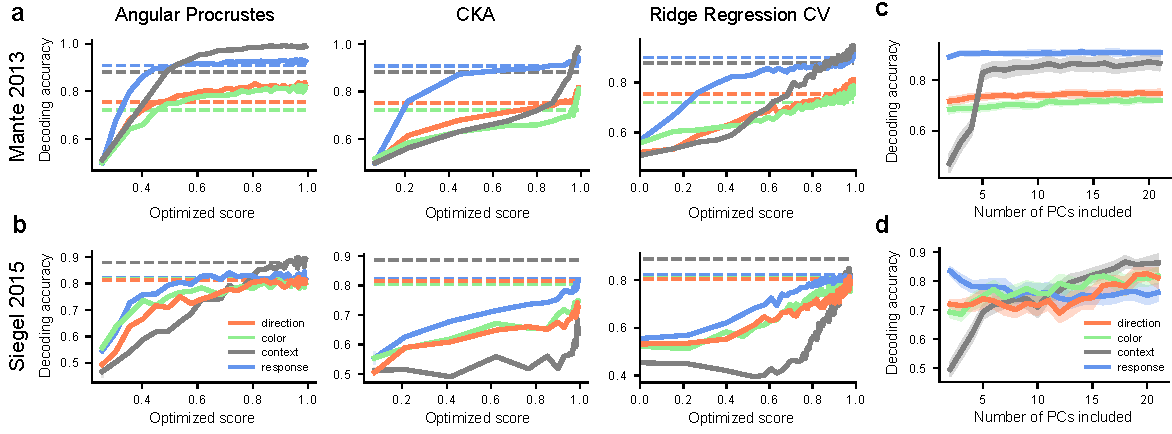
\includegraphics[width=\textwidth]{figures/var_decoding_without_condavg.pdf}
    \caption{\textit{(a, b)} \textbf{Decode accuracy for experimental variables versus similarity scores.} Decode is from synthetic data optimized towards greater similarity with the neural data from \textit{(a)} \citet{Mante2013} and \textit{(b)} \citet{Siegel2015}. Horizontal dashed lines indicate the decode accuracy from the neural data. \textit{(c, d)} Decode accuracy from neural data versus number of principal components included in the decode. Decode uses data from \textit{(c)} prefrontal cortex from Mante et al. 2013 and \textit{(d)} FEF from Siegel et al. 2015.}
    %\caption{b, d: stop optimization when reach 0.99 }
    \label{fig:var_decoding_supp}% To reference this figure in the main text use Figure \ref{fig:2}
    \myspaceafterfigures
\end{figure}


\begin{figure}[h!]
  \centering% to avoid extra vertical space use \centering instead of \begin{center} and \end{center}
    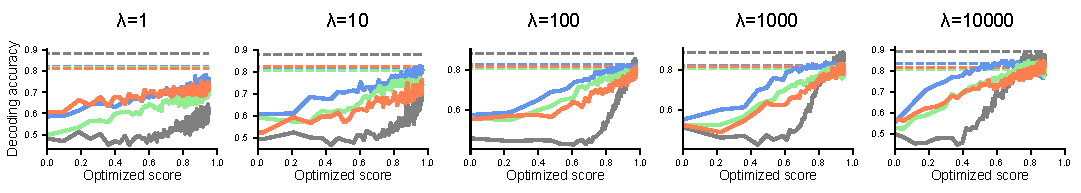
\includegraphics[width=\textwidth]{figures/linreg_comparison_without_condavg.pdf}
    \caption{\textbf{Decode accuracy versus similarity scores when optimizing ridge regression scores with varying regularization strengths} $\lambda$. Regression scores are cross-validated across conditions. Horizontal lines show the decode accuracy from the neural data for the task relevant variables, and colored curves shows the corresponding decode accuracy on a synthetic dataset that is optimized to become increasingly more similar to the neural data. For some values of the ridge regularization parameter, even at the highest similarity scores near 1, the synthetic dataset does not encode task relevant information to the same extent as the neural data.
}
    \label{fig:linreg_comparison}% To reference this figure in the main text use Figure \ref{fig:1}
\end{figure}



\begin{figure}[h!]
  \centering% to avoid extra vertical space use \centering instead of \begin{center} and \end{center}
    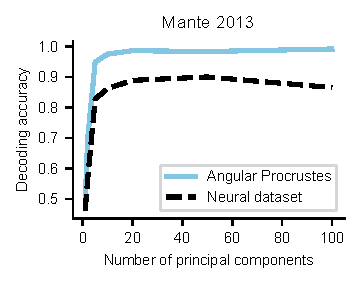
\includegraphics[width=0.38\textwidth]{figures/task_var_decoding_pca.pdf}
    \caption{
    We test whether removing low-variance principal components from the neural dataset increases the decoding accuracy, in order to see if this ``denoising'' may be a potential mechanism for explaining the increased decoding accuracy in the optimized dataset compared to the reference neural dataset in Figure~\ref{fig:3}. We show results for decoding of the context task variables from the Mante 2013 dataset after projecting onto principal components 1 through N, where principal component 1 is taken to have the highest variance, and N increases along the x-axis of the figure. The solid blue line shows the decoding accuracy from the synthetic dataset optimized with Angular Procrustes when the similarity score reaches a value of 0.9. %The increased decoding accuracy in the optimized datasets persist even when denoising the neural dataset with PCA. 
    %The decode accuracy from the neural dataset does not match the value for the synthetic data when lower variance components are removed. 
    Although the decoding accuracy from the neural data increases slightly when the lowest variance components are removed, it does not match the decoding accuracy from the synthetic data. %This suggests it is probably a more complex form of denoising and would require further investigation. 
    This suggests the improved decoding accuracy from the synthetic data is probably a more complex form of denoising and would require further investigation.
    }
    \label{fig:task_var_decoding_pca}% To reference this figure in the main text use Figure \ref{fig:1}
\end{figure}


\section{Neural Datasets and Models} \label{appendix:models_and_datasets}

% \subsection{Tasks and datasets}
% We compare neural firing rates and RNN activity across three tasks: a contextual decision making task with electrode recordings from prefrontal cortex (PFC) \citep{Mante2013}, a maze reaching task with electrode recordings from primary motor (M1) and dorsal premotor cortex (PMd) \citep{Sussillo2015}, and a center-out reaching task with electrode recordings from M1 \citep{Hatsopoulos2007}. However, the approach is designed to be scalable to many more datasets.\\
\subsection{Datasets} \label{appendix:datasets}

We analyzed neural data from five studies on nonhuman primates:
\begin{itemize}
    \item \citet{Mante2013}: Prefrontal cortex (PFC) electrode recordings during a contextual decision-making task involving colored moving dots. Activity is averaged across trials with the same condition (72 unique conditions) and averaged across 50 ms non-overlapping time bins during the 750 ms interval from 100 ms after dots onset to 100 ms after dots offset. The total number of neurons recorded is 727. To make optimization faster, we reduce the dimensionality of this dataset by keeping 99\% of the variance, corresponding to the first 448 principal components. Data link\footnote{ \url{https://www.ini.uzh.ch/en/research/groups/mante/data.html}}. The final dataset used in all the similarity analyses had size (time = 15, sample = 72, feature = 448).
    \item \citet{Siegel2015}: Electrode recordings from multiple cortical regions during a contextual decision-making task involving colored moving dots, similar to Mante et al. (2013). We analyze data from the Frontal Eye Field (FEF) region during the stimulus period of the task. Activity is averaged across trials with the same condition (42 unique conditions) and averaged across 50 ms non-overlapping time bins from 0 to 500 ms after dots onset. A total of 1220 neurons were recorded. We reduce the dimensionality of this dataset by keeping 99\% of the variance, corresponding to the first 278 principal components. The final dataset used in all the similarity analyses had size (time = 11, sample = 42, feature = 278).
    \item \citet{Hatsopoulos2007}: Primary motor (M1) electrode recordings during a center-out reaching task. Simultaneous recordings were collected for 391 trials, 141 neurons. Activity is averaged across 50 ms non-overlapping time bins from 0 to 500 ms after movement onset. Data link\footnote{\url{https://datadryad.org/stash/dataset/doi:10.5061/dryad.xsj3tx9cm}}. The final dataset used in all the similarity analyses had size (time = 10, sample = 391, feature = 141).
    \item \citet{MajajHong2015}: Inferior temporal (IT) electrode recordings during object image presentations. Simultaneous recordings for 3200 trials, 168 neurons. Activity is averaged across all time steps. The final dataset used in all the similarity analyses had size (sample = 3200, feature = 168).
    % "Our goal was to assess neuronal activity patterns that are automatically evoked by presenting a visual image to an awake, alert visual system. Therefore, the monkey's only task was to maintain gaze on a fixation dot in the middle of a screen for 2–4 s as images were serially presented at the center of gaze. The monkeys initiated each trial by fixating a central red square." Majaj, Hong et al. 2015
    \item \citet{Freeman2013}: Primary (V1) and secondary (V2) visual area electrode recordings during texture and noise image presentations. Simultaneous recordings were collected for 135 trials, 205 neurons. Data is averaged across 150 ms non-overlapping time bins. The final dataset used in all the similarity analyses had size (time = 2, sample = 135, feature = 205).
\end{itemize}
We use the BrainScore\footnote{\url{https://github.com/brain-score/vision}} library \citep{Schrimpf2020integrative} for the \citet{MajajHong2015, Freeman2013} datasets.



\subsection{Recurrent Neural Network (RNN) models}
\textbf{RNN architectures.}
We show results for three commonly used RNN architectures: LSTMs \citep{HochreiterSchmidhuber1997} and two choices for continuous time recurrent neural networks (CTRNNs), which differ by the position of the nonlinearity \citep{KennethMiller2012}. A first alternative is given by the following equations.
% \begin{align*}
% \tau \dfrac{dh}{dt} &= -h + Wr + Bu + b\\
% r &= f(h) + \xi
% \end{align*}
$$
\left\{
    \begin{array}{ll}
        \tau \dfrac{dh}{dt} = -h + Wr + Bu + b\\
        r = f(h) + \xi
    \end{array}
\right.
$$
where $u$ is the input, $h$ represents the membrane potential, $\xi$ is a Gaussian white noise, and $r$ is the firing rate produced by the model and is used to compare the model with the neural data. The second alternative is given by the following equation.
$$\tau \dfrac{dr}{dt} = -r + f(Wr + Bu + b) + \xi$$
We call it the LowPassCTRNN since it can be shown that its firing rate is a low-pass filter of the firing rate of the first architecture, which we call CTRNN \citep{KennethMiller2012}. The RNNs are trained using supervised learning on simplified task inputs and outputs.\\

\textbf{Comparing task-optimized RNNs to neural datasets.}
We train the RNNs on the tasks from \citet{Mante2013} and \citet{Siegel2015}, and compare them to the respective neural datasets.
We consider two neural datasets from prefrontal cortex (PFC) \citep{Mante2013} and Frontal Eye Field (FEF) \citep{Siegel2015} in monkeys performing an experimental task that required the animal to attend to either color or motion information while ignoring the non-cued feature of the stimuli. 
On each trial, a field of colored moving dots is shown.  Monkeys are given a cue at the beginning of the trial to determine whether the dots in the stimulus are moving left vs right, or are red vs green. The monkey reported its choice with a saccade to one of two visual targets. In both datasets, we analyzed neural activity taken when the dot stimulus was presented. In panel \textit{a} of Figure \ref{fig:rnn} neural activity is visualized in a low-dimensional space capturing task-relevant dynamics using the targeted dimensionality reduction method from Mante et al. 2013. Each curve shows the average neural activity for a different experimental condition. See Mante et al. 2013 for a detailed description of the analysis. This visualization highlights features of the data but the similarity scores were computed using the firing rates from the electrode recordings before any dimensionality reduction. In panel \textit{b} of Figure \ref{fig:rnn} neural firing rates for two example neurons are shown with the colors denoting average.

In Figure \ref{fig:rnn} \textit{c, d}, we compare model-data similarity scores to two baseline scores.
The Neuron-split baseline score is obtained by dividing the neurons from a single dataset into disjoint sets and then comparing. If the model-data scores are equal to the neuron-split scores this indicates that model activity is indistinguishable from the neural activity of other recorded neurons. 
The Condition-average baseline score is obtained by averaging the neural activity along the trial and condition dimensions and comparing it to the original dataset. Each neuron in this condition-averaged dataset still has a unique time-varying firing rate. This strong baseline shows the similarity to the original data that one can obtain by only keeping the condition-independent neural dynamics. 


% \subsection{Condition average baseline:} 
% The condition average baseline is obtained by averaging the neural activity along the condition dimension, while still allowing each neuron to have its own unique time-varying firing rate, and then comparing this condition-averaged dataset to the original neural data. This baseline shows the similarity one can obtain by discarding the condition specific activity to keep only the condition independent dynamics of the neural activity. 



\section{Similarity Measures} \label{appendix:similarity_measures}

% Optionally include supplemental material (complete proofs, additional experiments and plots) in appendix.
% All such materials \textbf{SHOULD be included in the main submission.}

\subsection{Definitions} \label{appendix:measures}

Several methods have been proposed to measure similarity between models and neural data (see \citep{sucholutsky2023getting}, \citep{klabunde2023similarity} for comprehensive reviews). 
While some efforts have been made to characterize these metrics mathematically, for instance, by examining their invariance properties, clear guidance in interpreting similarity scores for a given scenario remains limited. %clear guidance on selecting the most appropriate metric for a given scenario remains limited. 
To address this gap, we introduce a novel method for analyzing the specific aspects of data prioritized by different similarity metrics. Our method leverages the differentiability of these metrics and is applicable to a wide range of measures.
We focus here on three commonly used metrics and their variants, linear regression \citep{YaminsHong2014, SchrimpfKubilius2018}, Centered Kernel Alignment (CKA) \citep{Kornblith2019}, and Procrustes distance \citep{Williams2021, ding2021grounding}. 
These methods quantify similarity based on the goodness of fit after aligning the representations. This alignment transformation allows for greater flexibility by making similarity measures invariant to specific transformations. For example, instead of demanding a one-to-one mapping of neurons between datasets, these methods can accommodate scenarios where neurons in one dataset correspond to linear combinations of neurons in the other.
% These methods quantify similarity by measuring a goodness of fit after allowing for some alignment of the representations. Intuitively, the alignment transform allows similarity measures to be more flexible or in other terms to be invariant to specific transformations. For example, it can be used to allow neurons in one dataset to correspond to combinations of neurons in the other dataset, which is less strict than requiring a one to one mapping of the neurons for example.

Consider two datasets $X$ and $Y$ with shape (sample, feature) and mean-centered columns. Datasets with dynamics are shaped from (time, sample, feature) to (time*sample, feature).

Assuming $X$ as our reference dataset (e.g., neural data), linear regression seeks the optimal linear mapping $B$ to predict $X$ from $Y$. We use the $R^2$ coefficient to evaluate goodness of fit and ridge regularization with parameter $\lambda = 100$, as well as 5-fold cross-validation. Note that we apply cross-validation after reshaping the data from (time, sample, feature) to (time*sample, feature).
% $$R^2_{LR} = 1 - \dfrac{\min_B \| X - YB\|^2_F + \lambda \| B \|_F}{\| X \|^2_F}$$

$$B^* = \argmin_B \| X - YB\|^2_F + \lambda \| B \|_F$$

$$R^2_{LR} = 1 - \dfrac{\| X - YB^*\|^2_F}{\| X \|^2_F}$$

It's important to note that this score is not symmetric. Applying linear regression on $Y$, $X$ instead of $X$, $Y$ may yield significantly different scores. This asymmetry arises because one dataset might be highly predictive of the other, while the reverse might not hold true.

% from Brian Cheung's paper: "Recent work (Diedrichsen et al., 2020) notes that linear CKA is equivalent to a whitened representational dissimilarity matrix (RDM) in RSA under certain conditions "

Unlike linear regression, CKA and Procrustes are symmetric, meaning the metric yields the same result whether applied to X, Y or Y, X. 
Moreover, they exhibit a different class of invariance.
While linear regression is invariant under invertible linear transformations, CKA and Procrustes are invariant under orthogonal linear transformations. This stricter invariance to orthogonal transformations potentially reduces sensitivity to noise \citep{Kornblith2019}.

CKA measures the correlation between the kernels of two datasets $X$ and $Y$ \citep{Kornblith2019}. We consider here linear CKA where the kernels are $XX^T$ and $YY^T$.
% $$\text{CKA}(X, Y) = \dfrac{\| X^T Y \|^2_F}{\| X X^T \|_F \| Y Y^T \|_F}$$
$$\text{CKA}(X, Y) = \dfrac{\langle \text{vec}(XX^T), \text{vec}(YY^T) \rangle}{\|XX^T\|_F \| YY^Y\|_F} = \dfrac{\| X^T Y \|^2_F}{\| X X^T \|_F \| Y Y^T \|_F}$$

CKA scores range from 0 to 1, with 1 indicating perfect similarity. 
% We also consider another variant of CKA which is the arccosine of CKA. As \citep{Williams2021} showed, this gives a measure of distance, where 0 corresponds to perfect similarity, that satisfies the axioms of a metric, e.g. the triangle inequality. 
We also consider the arccosine of CKA, a metric satisfying the axioms of a distance metric (e.g., the triangle inequality) with 0 signifying perfect similarity \citep{Williams2021}.
This metric, also known as Angular CKA \citep{lange2022neural}, is then normalized to a similarity score between 0 and 1 for direct comparison with other scoring methods. This normalization involves dividing the angular distance by $\pi/2$ and subtracting the result from 1, ensuring the measure increases with similarity.
% This metric has been also called Angular CKA as \citep{lange2022neural}. Here we normalize this meause to have a measure of similarity between 0 and 1 so that it can directly be compared to other scoring methods. We do that by first normalizing the angular distnace between 0 and 1 by dividing by pi over 2, and then substract the result from 1 to have a measure that increases with similarity.
$$\text{AngularCKAScore}(X, Y) := 1 - \dfrac{\arccos (\text{CKA}(X, Y))}{\pi / 2}$$

Procrustes distance provides another approach for quantifying similarity \citep{Williams2021, ding2021grounding}. This metric identifies the optimal orthogonal alignment to maximize the correlation between $X$ and $Y$:
% Another method to quantify similarity is the Procrustes distance \citep{Williams2021, ding2021grounding}. The Procrustes distance finds the best orthogonal alignment to maximize the correlation between $X$ and $Y$
$$\max_{Q \in \mathcal{O}} \dfrac{\langle X, QY\rangle}{\|X\|_F \|Y\|_F}$$
where $\mathcal{O}$ is the group of orthogonal linear transformations. An angular distance metric can be obtained by taking the arccosine of this quantity \citep{Williams2021}.

As shown in \citet{harvey2023duality}, Procrustes distance is closely related to Normalized Bures Similarity (NBS) \citep{tang2020similarity}, with Procrustes distance equating the arccosine of NBS. NBS is defined as:
$$\text{NBS}(X, Y) = \dfrac{\|X^T Y\|_*}{\sqrt{\|X X^T\|_* \|Y Y^T\|_*}}$$

This definition resembles CKA but utilizes the nuclear matrix norm instead of the Frobenius matrix norm.
The Frobenius norm, denoted by $\|A\|_F$ for a matrix $A$, is calculated as the square root of the sum of squared singular values. The nuclear norm, $\|A\|_*$, is simply the sum of singular values.
The implications of this difference in matrix norms for the weighting of principal components by CKA and NBS are further explored in \ref{appendix:cka_nbs_theory}.
% See \ref{appendix:cka_nbs_theory} for how this different in matrix norms can explain in how CKA and NBS differentially weight principals components of the data.


Similar to the score version of CKA distance, we define a score version of Procrustes distance, ranging from 0 to 1, where 1 represents perfect similarity.

$$\text{AngularProcrustesScore}(X, Y):= 1 - \dfrac{\arccos (\text{NBS}(X, Y))}{\pi / 2}$$


% One advantage of being invariant to orthogonal transformations instead of invertible linear, is that it is less sensitive to noise. An invertible linear transformation can scale each dimension arbitrarily. It can arbitrarily increase the magnitude of the activity along any dimension, even dimensions of low variance. This makes it susceptible to finding spurious correlation in low variance, noise dimensions.



% It is useful to think about the invariances that these similarity measures have. Since linear regression finds the best linear mapping, it means it is invariant to invertible linear transformation. The score between X and Y is the same as the score between X and YA, for any invertible matrix A. Another way to see this is that instead of asking how model to match exactly the activity of individual neurons in the brain, which might be too much to ask, we allow a unit of the model to match a linear combination of neurons in the brain.

% Procrustes has a more strict invariance class. It is invariant under orthogonal transformations, which is a subset of invertible linear transformations. Procrustes finds the orthogonal transformation that maximizes the correlation between the two datasets. The Procrustes distance can be seen as the residual dissimilarity that cannot be captured by just an orthogonal alignment.

% CKA is also invariant under orthogonal transformation.



% Looking at the invariance properties doesn't tell us the full story. Even though CKA and Procrustes have the same set of invariances, they exhibit very different behavior when used in practice. The analysis we present in this work aims at better characterizing what these measures care about practically.


% We take the convention that an increasing similarity score corresponds to increasing similarity, with a maximum value of 1 for perfect similarity. Before applying the similarity measures, the datasets are preprocessed by averaging the firing rates for trials with the same conditions. The results is an data array of shape $(\text{time}, \text{conditions}, \text{neurons})$, which still carries temporal information and differences across conditions. Most of the commonly used similarity measures operate on matrices. We reshape our 3d data array into a 2d matrix by concatenating the time and condition dimensions together, resulting in an array of shape $(\text{time}*\text{conditions}, \text{neurons})$. 




% Several methods have been proposed to measure similarity between models and neural data \citep{sucholutsky2023getting}, \citep{klabunde2023similarity}. Although the approach presented here can be applied to any differentiable similarity measure, we selected three commonly used methods, linear regression \citep{YaminsHong2014, SchrimpfKubilius2018}, CKA \citep{Kornblith2019}, and Procrustes distance \citep{Williams2021, ding2021grounding}.
% We take the convention that an increasing score corresponds to increasing similarity, with a maximum value of 1 for perfect similarity.




% link between CKA and Procrustes (different choice of matrix norm, CKA: sum of squared singular values, NBS: sum of singular values).

% \citep{ding2021grounding}, \citep{davari2022reliability}: CKA insensitive to perturbations in task-relevant lower variance PCs


% , \citep{lange2022neural}: Angular version of CKA (don't know if has the same issues as CKA). Here, normalized so that score of 1 corresponds to perfect similarity.




\subsection{Theoretical analysis of CKA and NBS} \label{appendix:cka_nbs_theory}
Our results show that similarity in the high variance components seem to dominate the Centered Kernel Alignment (CKA) score. In contrast, while the high variance components still have an overall larger impact than lower variance components, metrics like Normalized Bures Distance (NBS) seem to be more sensitive to changes in lower variance components relative to CKA. We explain this difference by showing, in theory, how CKA and NBS changes when perturbing a single principal component of the data. The result is that CKA depends quadratically on the variance of the perturbed principal component, whereas NBS has a linear dependence. We start the derivation from the matrix norm definitions of CKA and NBS \citep{harvey2023duality}.
$$\text{NBS}(X, Y) = \dfrac{\|X^T Y\|_*}{\sqrt{\|X X^T\|_* \|Y Y^T\|_*}}$$
$$\text{CKA}(X, Y) = \dfrac{\| X^T Y \|^2_F}{\| X X^T \|_F \| Y Y^T \|_F}$$


Let $X$ be a dataset, and $Y$ be a perturbed version of $X$, denoted $\tilde{X}_k$, where only the $k^{\text{th}}$ principal component is modified. Specifically, define $Y$ such that its $j^{\text{th}}$ left singular vector $u_Y^j$ is equal to the $j^{\text{th}}$ left singular vector $u_X^j$ of $X$ for all $j \neq k$, and define $u_Y^k$ to be a perturbation of $u_X^k$ that preserves variance. Here we randomly sample $u_Y^k$ from a Gaussian distribution with the same variance as the variance of $u_X^k$ so that $\sigma_Y^k = \sigma_X^k$. The right singular vectors of $Y$ are the same as the right singular vectors of $X$. Intuitively this perturbation affects only the projection of the data along the $k^{th}$ principal component.

We first show how $\text{CKA}(X, \tilde{X}_k)$ depends on the variance of the perturbed principal component. As shown in \citep{Kornblith2019}, CKA can be rewritten in terms of dot products of the left singular vectors.

$$\text{CKA}(X, Y) = \dfrac{\sum_{i, j} \lambda_X^i \lambda_Y^j \langle u_X^i, u_Y^j \rangle^2}{\sqrt{\sum_i (\lambda_X^i)^2}\sqrt{\sum_j (\lambda_Y^j)^2}}$$

where $X = U_X\Sigma_X V^T_X$, $Y = U_Y\Sigma_Y V^T_Y$ are the SVD decompositions of $X$ and $Y$ respectively, and $\lambda_X^i = (\sigma_X^i)^2$, $\lambda_Y^i = (\sigma_Y^i)^2$. Since $u_Y^j = u_X^j$ for all $j \neq k$ and since $U_X$ is an orthogonal matrix, the dot products $\langle u_X^i, u_Y^j \rangle$ are equal to $0$ for all $j \ne i$ whenever $j \ne k$. The dot products $\langle u_X^i, u_Y^k \rangle$ are not guaranteed to be zero since randomly sampling $u_Y^k$ doesn't guarantee to preserve the orthogonality with the other left singular vectors. However, when the number of samples in the data is large the projection $u_Y^k$ on the other singular vectors will be relatively small. With the assumption that $\langle u_X^i, u_Y^k \rangle \approx 0$, CKA can be written as:

$$\text{CKA}(X, \tilde{X}_k) \approx \dfrac{\sum_{i \ne k} (\lambda_X^i)^2}{\sum_i (\lambda_X^i)^2}$$


This shows that CKA scores between the original data and the perturbed data depend quadratically on the variance of the perturbed principal component. As shown in Figure \ref{fig:theory_all_datasets}, our theoretical approximation closely matches simulations.


As opposed to CKA, NBS cannot be directly rewritten as a sum of left singular vector dot products. However, we show that NBS reduces to a simple form when $Y$ is defined as $X$ perturbed along a single principal component and when $\langle u_X^i, u_Y^k \rangle \approx 0$ is assumed. We start by expressing the nuclear norm in the numerator of NBS in terms of the SVD decomposition of $X$ and $Y$.

$$\|X^TY\|_* = \|V_X\Sigma_XU^T_X U_Y\Sigma_Y V^T_Y \|_* = \|\Sigma_XU^T_X U_Y\Sigma_Y \|_*$$

The individual entries of the product of matrices inside the nuclear norm corresponds to the dot products between the left singular vectors of $X$ and $Y$ weighted by the corresponding singular values.
$$[\Sigma_X U_X^T U_Y \Sigma_Y]_{ij} = \sigma^i_X \sigma^j_Y \langle u_X^i, u_Y^j \rangle$$

By definition of $Y \equiv \tilde{X}_k$,
$$
\sigma_X^i \sigma_Y^j \langle u_X^i, u_Y^j \rangle = \begin{cases} 
(\sigma_X^i)^2 \delta_{ij} & \text{if } j \neq k \\
\sigma_X^i \sigma_X^k \langle u_X^i, u_Y^k \rangle & \text{if } j = k 
\end{cases}
$$
With our assumption that $\langle u_X^i, u_Y^k \rangle \approx 0$ and the nuclear norm property $\|A\|_* = \text{Tr}\left[ \sqrt{A^T A} \right]$, we find:

$$\|X^TY\|_* \approx \sum_{i \ne k} (\sigma_X^i)^2$$

Since our perturbation preserves the variance, we have $\|XX^T\|_* = \|YY^T\|_* = \sum_i (\sigma_X^i)^2$. We finally obtain the following approximation, which explicitly reveals the linear dependence of NBS on the variance of the principal components.
$$\text{NBS}(X, \tilde{X}_k) \approx \dfrac{\sum_{i \ne k} (\sigma_X^i)^2}{\sum_i (\sigma_X^i)^2} = \dfrac{\sum_{i \ne k} \lambda_X^i}{\sum_i \lambda_X^i}$$



% $$\text{NBS}(X, \tilde{X}_k) \approx \dfrac{\sum_{i \ne k} \lambda_X^i}{\sum_i \lambda_X^i}$$

% $$\|A\|_* = \sum_i \sigma_i(A)$$
% $$\|A\|_F = \sqrt{\sum_i \sigma_i(A)^2}$$

% $$\text{AngularProcrustes}(X, Y)= 1 - \arccos (\text{NBS}(X, Y)) / \frac{\pi}{2}$$


% might not have time to explain this in this version
% \section{Similarity Repository}
% TODO: explain structure of similarity-repository package

% \begin{figure}[h]
%     \centering% to avoid extra vertical space use \centering instead of \begin{center} and \end{center}
%     \includegraphics[width=\textwidth]{figures/backends_matrix.png}
%     \caption{TODO: implement more variants in diffscore. Replace repo name by paper name?}
%     \label{fig:enter-label}% To reference this figure in the main text use Figure \ref{fig:enter-label}
% \end{figure}


% added based on the rebuttals
\subsection{Joint optimization of similarity measures} \label{appendix:joint_optim}
Figure \ref{fig:joint_optim} shows how two metrics relate by jointly optimizing for both metrics. Given a score for the first metric and a score for the second metric, we ask whether it is possible to find a single synthetic dataset that would produce these two similarity scores. Specifically, for a given reference dataset $X$, similarity measures $A$ and $B$, and respective targets $\text{target}_{\text{A}}$ and $\text{target}_{\text{B}}$, we optimize a synthetic dataset $Y$ to minimize the sum of absolute errors:
$$\min_Y \Big[ |\text{score}_{\text{A}}(X, Y) - \text{target}_{\text{A}}| + |\text{score}_{\text{B}}(X, Y) - \text{target}_{\text{B}}| \Big]$$

We chose the absolute error instead of the squared error as we find in practice that it gives scores that are closer to their targets.
% Practically, instead of optimizing a randomly initialized synthetic dataset to optimize a single similarity metric, we now jointly optimize for two similarity metrics. 

This analysis gives an approximation of the range of scores that two metrics can jointly take. For example, if two metrics are completely independent, then any point on the $[0, 1] \times [0, 1]$ square is reachable (see third plot of Figure \ref{fig:joint_optim}b for an example). However, if there exists a one-to-one mapping between the two metrics, then the scores are constrained to lie on a one-dimensional curve.


\begin{figure}[h!]
  \centering
    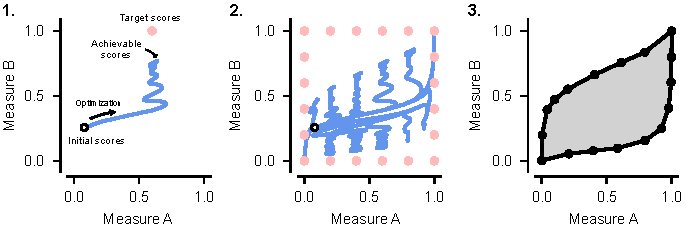
\includegraphics[width=\textwidth]{figures/joint_optim_explanation.pdf}
    \caption{\textbf{Computing the allowed ranges between two similarity scores by optimizing synthetic data towards a grid of target similarity scores.} \textit{(1)} 
    Given a synthetic dataset $Y$ and a reference dataset $X$ we attempt to simultaneously achieve the desired target scores for similarity measures A and B (pink circle). To do this we optimize $Y$ with the Adam optimizer by differentiating through the scores for similarity measure A, $\text{score}_{\text{A}}(X, Y)$, and B, $\text{score}_{\text{B}}(X, Y)$, to minimize a sum of absolute error loss function between the current and target similarity scores. As $Y$ is optimized the scores for measures A and B trace out the curve shown in blue. Note that the final achievable scores for the two similarity measures approach but, in this case, do not reach the target scores. \textit{(2)} This optimization procedure is repeated for many different target scores (pink dots) and the intermediate scores are recorded (blue curves). \textit{(3)} The edges of the blue curves are marked with black dots and approximate a boundary of achievable scores as shown in gray.} 
    \label{fig:joint_optim_explanation}
\end{figure}

\begin{figure}[h!]
  \centering
    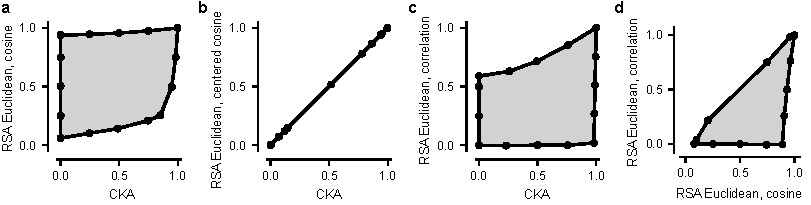
\includegraphics[width=\textwidth]{figures/joint_optim_rsa.pdf}
    \caption{\textbf{We analyze different variations of Representational Similarity Analysis (RSA) \citep{Kriegeskorte2008rsa} and CKA by jointly optimizing the similarity measures to approximate the allowable regions of scores.} \textit{(a)} We compare CKA and a commonly used version of RSA that uses the Euclidean distance to compute the Representational Dissimilarity Matrices (RDMs) and cosine similarity to compare the RDMs. We find that these two similarity measures are mostly independent, where a high score for one measure doesn't necessarily imply a high score for the other. \textit{(b)} We confirm the equivalence between CKA and RSA when centering the Euclidean RDMs before computing the cosine similarity, as shown by \citet{williams2024equivalence}. \textit{(c)} We compare CKA to another common variation of RSA that computes the correlation between the RDMs instead of the cosine similarity. We find that these two measures are also mostly independent. \textit{(d)} We compare two RSA variants together and show that changing the RDM comparison method makes the RSA measures non-equivalent.} 
    \label{fig:joint_optim_rsa}
\end{figure}

% RSA is indeed widely used and interesting to consider as there are many existing variants. We have now included a figure comparing common variants of RSA with CKA (Supplementary Figure S3). In particular, our new results confirm the equivalence between RSA with Euclidean RDMs and centered cosine similarity (see Williams UniReps 2024). However, they also show that other variations of RSA are almost independent of CKA, and that they might not even be equivalent to each other (as illustrated by comparing RSA with Euclidean RDMs using either cosine similarity or correlation to compare the RDMs).

\end{document}
